\documentclass[12pt]{book}
\usepackage[utf8]{inputenc}
\usepackage[T1]{fontenc}
\usepackage{tocbibind}
\usepackage{mathptmx}
\usepackage{geometry}
\usepackage{mathtools}
\usepackage[english]{babel}
\usepackage{graphicx}
\usepackage{subcaption}
\usepackage{stackengine}
\usepackage[os=win]{menukeys}
\usepackage{hyperref}
\usepackage{xcolor}
\usepackage{color}
\usepackage{tikz}
\usepackage[yyyymmdd,hhmmss]{datetime}
\usepackage{etoolbox}
\usepackage[inline]{enumitem}
\usepackage{listings}
\usepackage{booktabs}
\usepackage[os=win]{menukeys}

\newcommand{\WindowsLogo}{\raisebox{-0.1em}{
\includegraphics[height=0.8em]{images/logo/Windows_3_logo_simplified}}}
%\newcommand{\PowerLogo}{\raisebox{-0.1em}{
\includegraphics[height=0.8em]{images/logo/power}}}
\newcommand{\WinKey}{\keys{\WindowsLogo}}
\newcommand{\PowerKey}{\keys{\PowerLogo}}

%%%%% Mengganti label "Contents" ke "Daftar Isi" %%%%%
\addto\captionsenglish{\renewcommand{\contentsname}{Daftar Isi}}

%%%%% Mengganti label "Chapter" ke "Bab" %%%%%
\addto\captionsenglish{\renewcommand{\chaptername}{Bab}}

%%%%% Mengganti label "Figure" ke "Gambar" %%%%%
\addto\captionsenglish{\renewcommand{\figurename}{Gambar}}

%%%%% Mengganti label "List of Figures" ke "Daftar Gambar" %%%%%
\addto\captionsenglish{\renewcommand{\listfigurename}{Daftar Gambar}}

%%%%% Mengganti label "Table" ke "Tabel" %%%%%
\addto\captionsenglish{\renewcommand{\tablename}{Tabel}}

%%%%% Mengganti label "List of Tables" ke "Daftar Table" %%%%%
\addto\captionsenglish{\renewcommand{\listtablename}{Daftar Tabel}}

\hypersetup{
	colorlinks=true, %set true if you want colored links
	linktoc=all,     %set to all if you want both sections and subsections linked
	linkcolor=blue,  %choose some color if you want links to stand out
	urlcolor=blue,   %url color
}

\geometry{
	a4paper,
	left=10mm,
	right=10mm,
	top=15mm,
	bottom=15mm,
}

\date{}

\hypersetup{citecolor=black}

\definecolor{LightGray}{gray}{0.95}

%\pagecolor[rgb]{0.1,0.1,0.1}
%\color[rgb]{1,1,1}

\lstset
{
	language=bash,
	breaklines=true,
	basicstyle=\tt\normalsize,
	frame = single
}

\begin{document}

	\frontmatter
	\begin{titlepage}
		\centering
		{\LARGE \bf Panduan Dasar Draft PCB Menggunakan KiCAD}
		\vfill
		{\Large Achmadi ST MT}
		\vfill
		
\includegraphics[width=250pt]{images/logo/logoviblab}
		\vfill
		\vfill
	\end{titlepage}

	%%%%%%%%%%%%%%%%%%%%%%%%%%%%%%%%%%%%%%%%%%%%%%%%%%%%%%%%%%%%%%%%%

	\newpage
	\tableofcontents
	\listoffigures
	\listoftables

	%%%%%%%%%%%%%%%%%%%%%%%%%%%%%%%%%%%%%%%%%%%%%%%%%%%%%%%%%%%%%%%%%

	%%%%%%%%%%%%%%%%%%%%%%%%%%%%%%%%%%%%%%%%%%%%%%%%%%%%%%%%%%%%%%%%%

	\newpage
	\chapter{Penggunaan Buku}

	\section{Umum}
	Buku ini dibuat dengan tujuan penggunaan utama sebagai panduan digital untuk mempermudah search dan copy-paste.
	Anda tidak perlu mencetak buku ini ke bentuk kertas.
	Seluruh navigasi buku ini diharapkan menggunakan klik ke hyperlink di Daftar Isi,
	atau menggunakan tampilan \textbf{Index} yang tersedia di \textbf{SideBar} program pembaca PDF yang anda gunakan.

	\section{Petunjuk}
	Beberapa petunjuk yang digunakan di buku ini:
	\begin{itemize}
		\item \textbf{Cetak Tebal}: Menginformasikan identifier (keyword, variabel, fungsi, alamat, nama file, dst) yang berada di suatu paragraf
		\item \textbf{TIPS:} Menginformasikan hal-hal yang dapat membantu atau pengetahuan tambahan.
		\item \textbf{PERINGATAN:} Menginformasikan hal-hal yang bener-benar harus diperhatikan.
		\item Bentuk \menu[,]{File,Save} dan \keys[,]{ctrl,s} menunjukkan klik menu dan tombol keyboard.
	\end{itemize}

	%%%%%%%%%%%%%%%%%%%%%%%%%%%%%%%%%%%%%%%%%%%%%%%%%%%%%%%%%%%%%%%%%

	\newpage
	\mainmatter
	\chapter{Program KiCAD}

	\section{Pengenalan}

	KiCAD adalah paket software EDA (Electronic Design Automation) yang dikembangkan untuk perancangan papan sirkuit elektronik tercetak (Printed Circuit Board atau PCB)
	secara professional yang bersifat gratis dan terbuka.

	KiCAD dapat disandingkan dengan perangkat perancangan PCB professional lain seperti Altium, Diptrace, EasyEDA, dan lainnya.
	KiCAD tersedia untuk sistem operasi Windows, GNU/Linux, dan MacOS.\\

	Berikut adalah tampilan 4 software utama dalam paket software KiCAD:
	\begin{figure}[!ht]
		\centering
		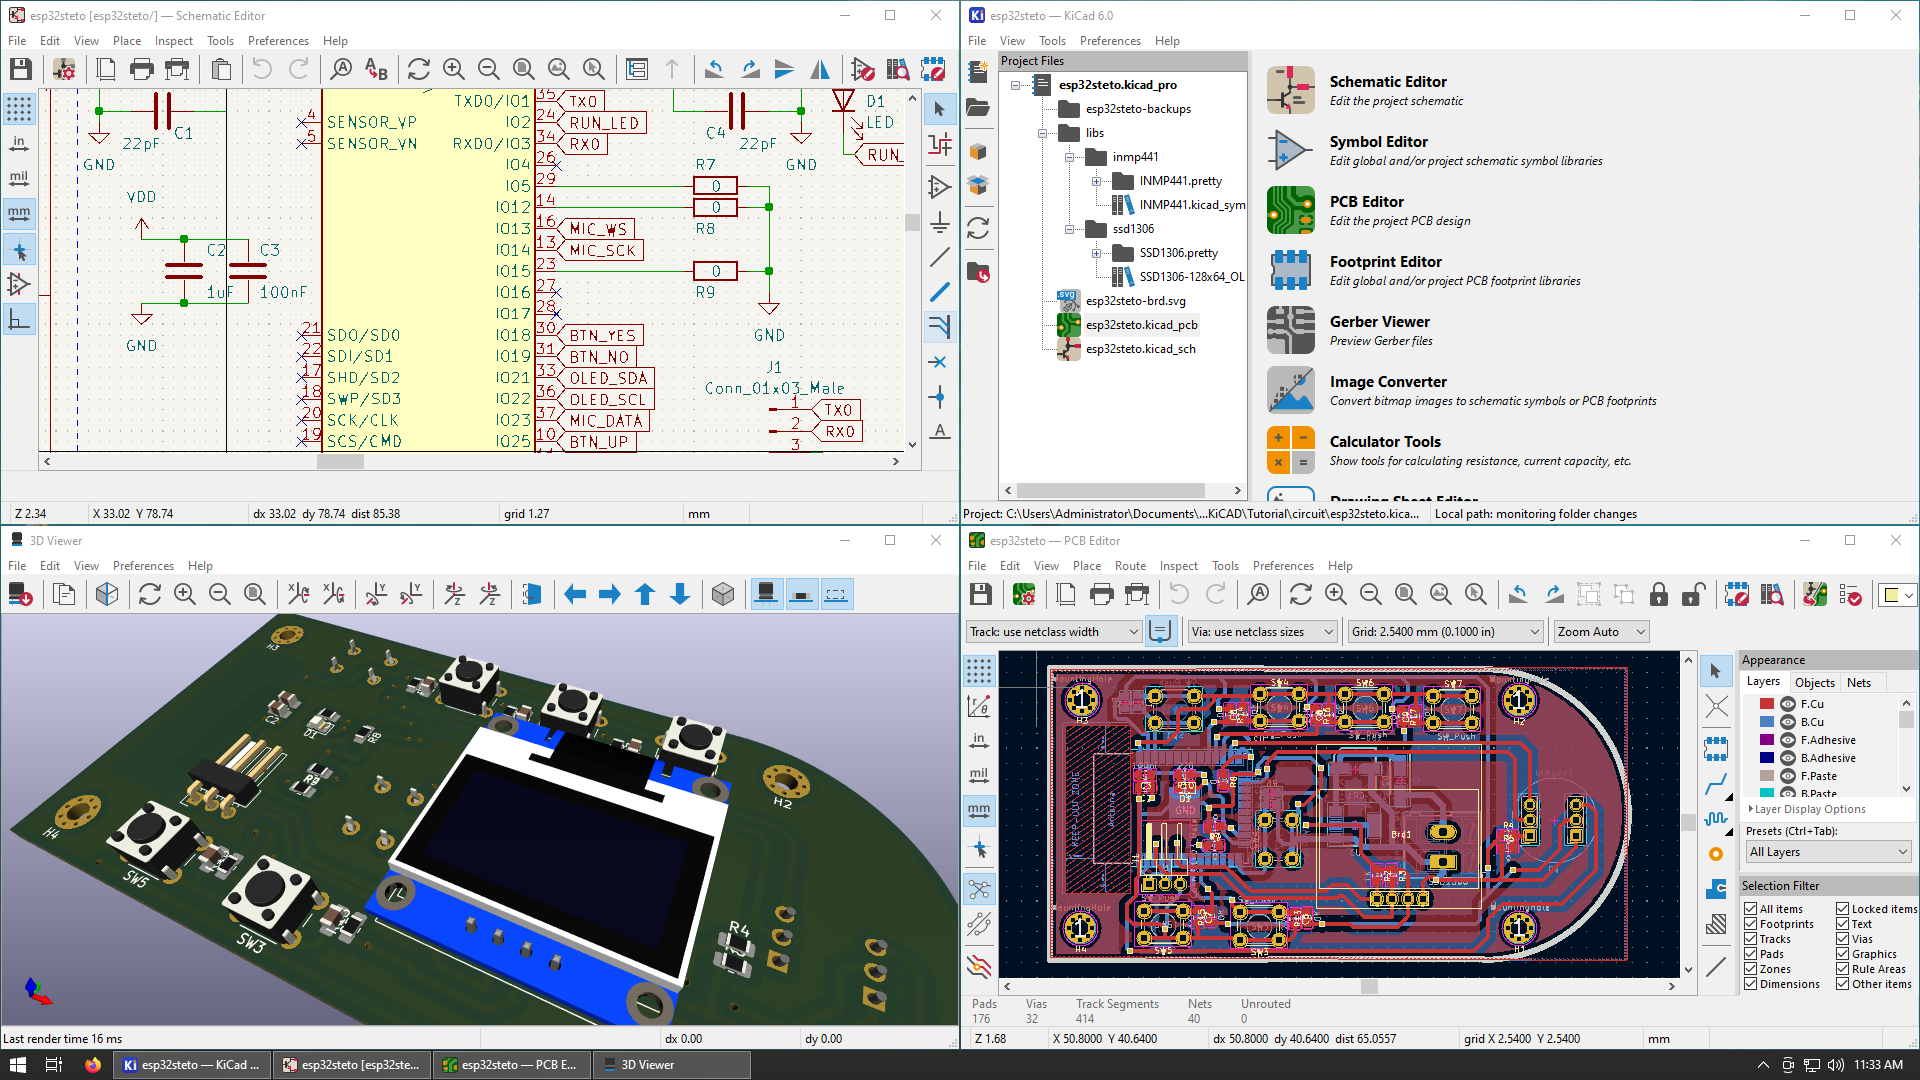
\includegraphics[width=\textwidth]{images/kicad_windows10}
		\caption{Tampilan KiCAD Windows 10}
	\end{figure}

	\textbf{TIPS:} Sepanjang tutorial, akan digunakan tampilan Windows 10 atau GNU/Linux sebagai acuan.
	Namun tutorial yang sama akan dapat pula digunakan di sistem operasi lain seperti Windows 8 dan Windows 11.\\

	\textbf{PERINGATAN:} Versi KiCAD yang akan digunakan adalah versi 6, dimana untuk sistem operasi Windows
	hanya bisa diinstal di Windows 8 dan selanjutnya.
	Untuk pengguna Windows 7 dan sebelumnya, disarankan menggunakan KiCAD versi 5.

	\newpage
	\section{Instalasi}

	\subsection{GNU/Linux}

	Berikut panduan instalasi KiCAD untuk dua jenis GNU/Linux yang populer, yaitu:
	\begin{itemize}
		\item Arch based, seperti Arch-Linux dan Manjaro.
		\item Ubuntu based, seperti Ubuntu-Mate dan Xubuntu.
	\end{itemize}

	\textbf{TIPS:} Untuk sistem operasi GNU/Linux, semua instalasi dilakukan via perintah di
	terminal emulator dengan sumber paket instalasi adalah mirror terdekat dari repository server masing-masing sistem operasi.\\

	\textbf{TIPS:} Perlu diingat untuk instalasi di GNU/Linux dibutuhkan hak akses administratif (umumnya sudo),
	sehingga dibutuhkan password akses tersebut.

	\subsubsection{Arch based}

	Untuk instalasi software KiCAD dan pustaka dasar, perintahnya adalah:

	\begin{lstlisting}
sudo pacman -S kicad kicad-library
	\end{lstlisting}

	Ukuran download berkisar 70MB dan ukuran instalasi berkisar 400MB.\\

	Kemudian untuk instalasi pustaka model komponen 3D, perintahnya adalah:

	\begin{lstlisting}
sudo pacman -S kicad-library-3d
	\end{lstlisting}

	Ukuran download berkisar 350Mb dan ukuran instalasi berkisar 5GB.\\

	\textbf{TIPS:} Jika diperlukan, lakukan update/upgrade sistem operasi dengan perintah:

	\begin{lstlisting}
sudo pacman -Syu --noconfirm
	\end{lstlisting}

	\subsubsection{Ubuntu based}

	Untuk instalasi KiCAD pada sistem operasi ini, digunakan sumber PPA khusus KiCAD 6:\\
	\url{https://launchpad.net/~kicad/+archive/ubuntu/kicad-6.0-releases} \\

	Pertama, tambahkan repository tersebut dengan perintah:
	\begin{lstlisting}
sudo add-apt-repository ppa:kicad/kicad-6.0-releases
sudo apt update
	\end{lstlisting}

	Kemudian perintah untuk instalasi seluruh paket lengkap (termasuk pustaka komponen 3D):
	\begin{lstlisting}
sudo apt install --install-recommends kicad
	\end{lstlisting}
	Ukuran download berkisar 500GB dan ukuran instalasi berkisar 6GB.\\

	Jika ingin menghindari paket komponen 3D dan menghemat ukuran instalasi, ganti perintah menjadi:

	\begin{lstlisting}
sudo apt install --install-recommends kicad kicad-library-packages3d-
	\end{lstlisting}

	\textbf{TIPS:} Jika memilih sistem operasi berbasis Ubuntu, disarankan memilih versi Ubuntu LTS dibandingkan
	reguler release.\\

	\textbf{PERINGATAN:} Hingga waktu penulisan tutorial ini, penulis hanya sebatas menggunakan
	KiCAD di Windows 10 dan Arch-Linux.
	Penulis belum mencoba pada sistem operasi Ubuntu.

	\newpage
	\subsection{Windows}

	Berikut panduan instalasi KiCAD untuk Windows 8, Windows 10, dan Windows 11.

	\subsubsection{Download}

	Installer KiCAD untuk Windows dapat didownload di alamat:\\
	\url{https://github.com/KiCad/kicad-source-mirror/releases}\\

	Atau spesifik untuk versi 6.0.7 untuk 64-bit dialamat:\\
	\url{https://github.com/KiCad/kicad-source-mirror/releases/download/6.0.7/kicad-6.0.7-x86_64.exe}\\

	\begin{figure}[!ht]
		\centering
		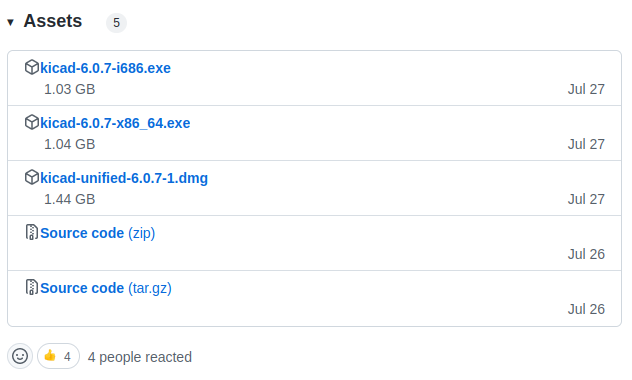
\includegraphics[width=0.75\textwidth]{images/installations/kicad_github}
		\caption{Download KiCAD}
	\end{figure}

	Ukuran berkas instalasi berkisar 1GB.\\

	\textbf{TIPS:} Penulis hanya merekomendasikan sumber instalasi dari URL Github di atas.
	Selain merupakan sumber resmi, juga Github menyediakan kecepatan download cukup tinggi.\\

	\textbf{TIPS:} Jika dibutuhkan versi 5 (seperti untuk Windows 7), dapat dikunjungi alamat berikut:\\
	\url{https://downloads.kicad.org/kicad/windows/explore/stable}\\

	Tutorial ini hanya akan menjelaskan KiCAD versi 6.

	\newpage
	\subsubsection{Proses Instalasi}

	Jalankan program installer yang telah di didownload. Klik \menu{Next}

	\begin{figure}[!ht]
		\centering
		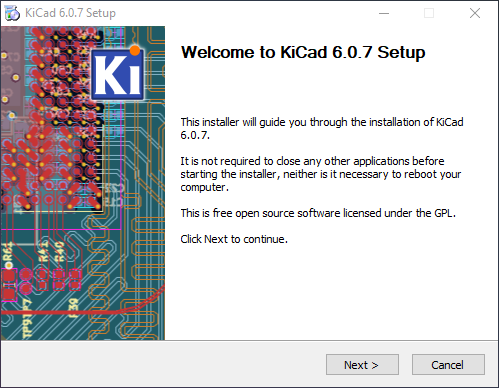
\includegraphics[width=0.7\textwidth]{images/installations/kicad_install_0}
		\caption{Memulai Instalasi KiCAD}
	\end{figure}

	Pilih paket apa saja yang ingin diinstal.
	Disini dapat di-\textit{unselect} paket Footprint 3D jika ada ingin menghemat 5GB instalasi.
	Lanjut klik \menu{Next}

	\begin{figure}[!ht]
		\centering
		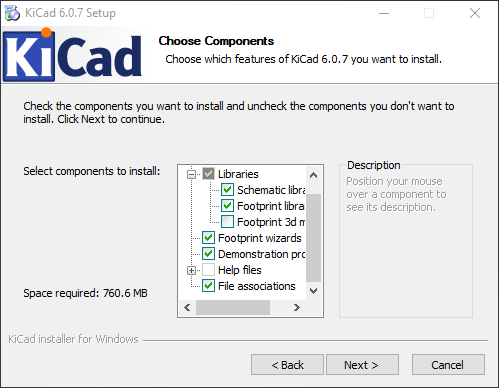
\includegraphics[width=0.7\textwidth]{images/installations/kicad_install_1}
		\caption{Pilih Paket}
	\end{figure}

	\newpage
	Tunggu proses instalasi hingga selesai

	\begin{figure}[!ht]
		\centering
		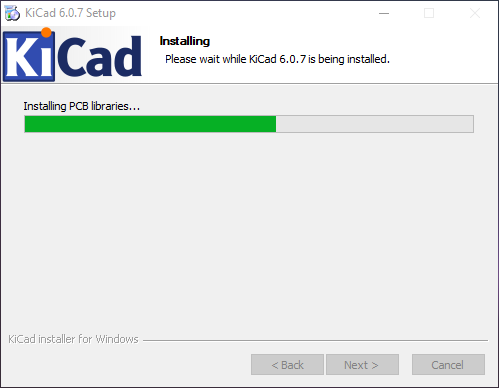
\includegraphics[width=0.7\textwidth]{images/installations/kicad_install_2}
		\caption{Proses Instalasi}
	\end{figure}

	Setelah instalasi selesai, dapat diklik \menu{Finish}.
	Tidak perlu install FreeCAD untuk saat ini.

	\begin{figure}[!ht]
		\centering
		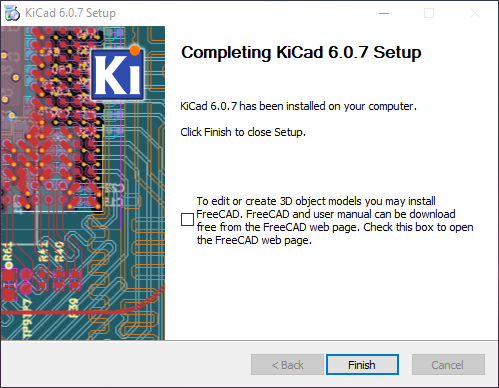
\includegraphics[width=0.7\textwidth]{images/installations/kicad_install_3}
		\caption{Instalasi Selesai}
	\end{figure}

	\newpage
	\subsection{MacOS}
	Nanti akan dilengkapi saat penulis cukup berduit untuk memiliki laptop Apple dan MacOS.

	\section{Memulai Program}

	Untuk memulai program KiCAD pada GNU/Linux, dapat digunakan perintah:
	\begin{lstlisting}
kicad
	\end{lstlisting}

	Atau dapat pula melalui menu sistem seperti pada sistem operasi Windows

	\begin{figure}[!ht]
		\centering
		\begin{subfigure}[t]{0.4\textwidth}
			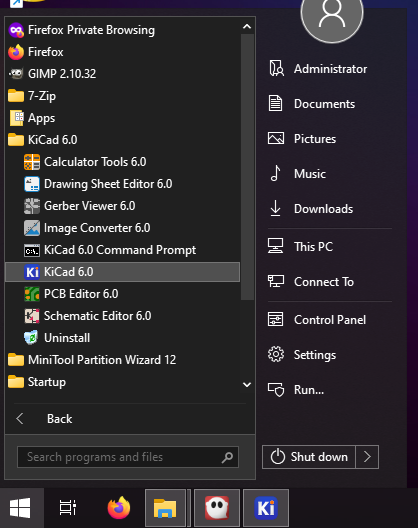
\includegraphics[width=\textwidth]{images/installations/kicad_menu_all}
			\caption{Windows 10}
		\end{subfigure}
		\begin{subfigure}[t]{0.4\textwidth}
			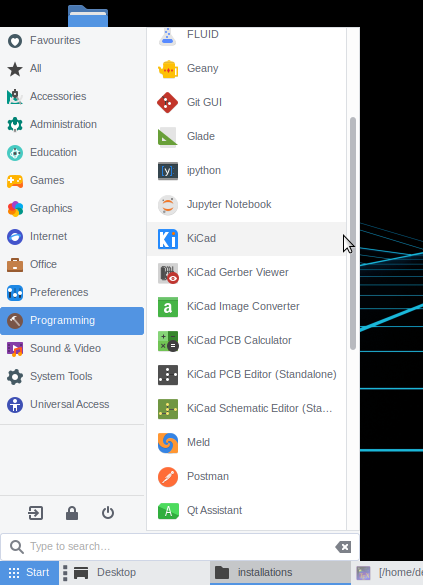
\includegraphics[width=\textwidth]{images/installations/kicad_menu_linux}
			\caption{Arch Linux}
		\end{subfigure}
		\caption{Memulai KiCAD via menu sistem operasi}
	\end{figure}

	Jika instalasi sukses, akan tampil pilihan migrasi pengaturan.
	Pilih default saja dan klik \menu{OK}.

	\begin{figure}[!ht]
		\centering
		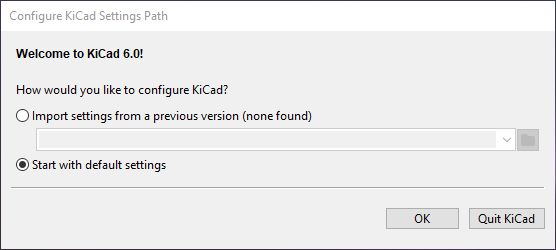
\includegraphics[width=0.7\textwidth]{images/installations/kicad_welcome}
		\caption{Migrasi Pengaturan}
	\end{figure}

	\newpage
	Tunggu beberapa saat, maka program utama KiCAD akan muncul.

	\begin{figure}[!ht]
		\centering
		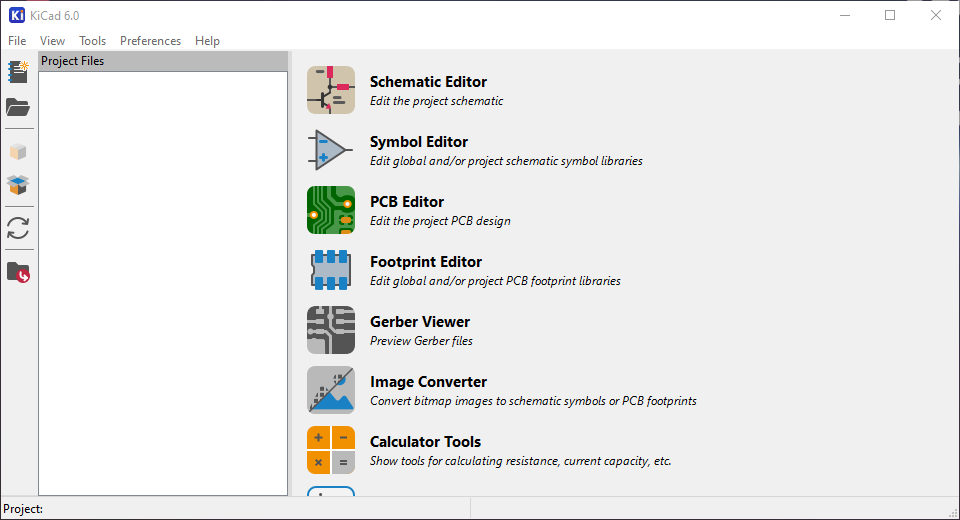
\includegraphics[width=\textwidth]{images/installations/kicad_first}
		\caption{Program Utama KiCAD}
	\end{figure}

	\textbf{PERINGATAN:} Jika saat menjalankan KiCAD muncul pesan OpenGL error seperti di bawah ini:

	\begin{figure}[!ht]
		\centering
		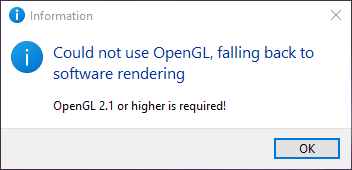
\includegraphics[width=0.7\textwidth]{images/installations/kicad_warn_noopengl}
		\caption{Peringatan OpenGL}
	\end{figure}

	Maka besar kemungkinan driver display atau VGA komputer masih menggunakan driver bawaan Windows.
	Silahkan update driver display komputer anda sesuai hardware yang terpasang.\\

	\begin{center}
		\textbf{Sampai disini, proses instalasi telah selesai.}
	\end{center}

	%%%%%%%%%%%%%%%%%%%%%%%%%%%%%%%%%%%%%%%%%%%%%%%%%%%%%%%%%%%%%%%%%

	\newpage
	\chapter{Dasar Konsep}

	\section{Program Utama}

	Berikut program utama KiCAD:

	\begin{figure}[!ht]
		\centering
		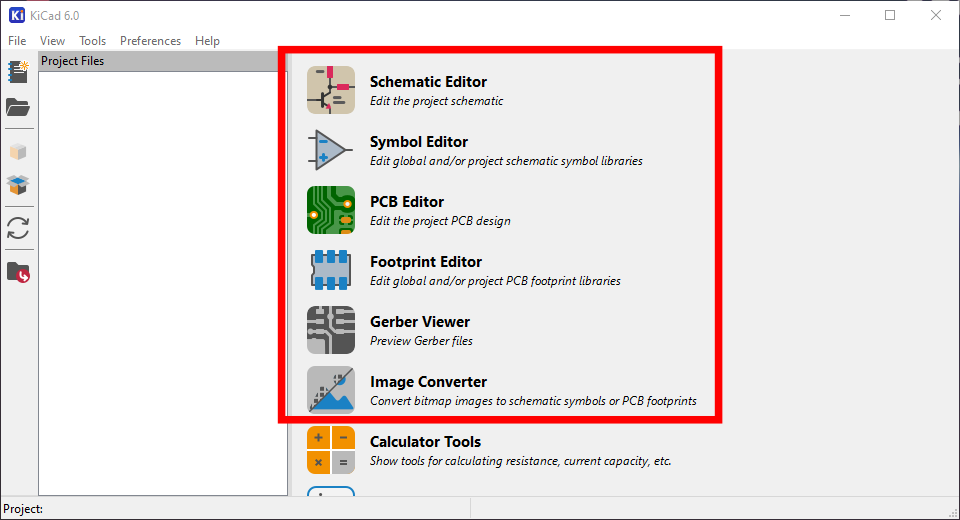
\includegraphics[width=\textwidth]{images/main/kicad_main}
		\caption{Program Utama KiCAD}
	\end{figure}

	Terdiri dari:
	\begin{itemize}
		\item \textbf{Schematic Editor}. Program menggambar skematik sirkuit.
		\item \textbf{Symbol Editor}. Program modifikasi atau membuat sendiri simbol komponen.
		\item \textbf{PCB Editor}. Program menggambar layout PCB.
		\item \textbf{Footprint Editor}. Program modifikasi atau membuat sendiri footprint (representasi aktual) komponen.
		\item \textbf{Gerber View}. Program menampilkan berkas-berkas Gerber
		\item \textbf{Image Converter}. Program mengkonversi gambar ke footprint
	\end{itemize}

	Mengingat ini adalah panduan dasar, maka Symbol Editor dan Footprint Editor tidak dibahas.

	\newpage
	\section{Workflow}

	Workflow proses perancangan PCB dengan KiCAD secara umum adalah seperti berikut:

	\begin{figure}[!ht]
		\centering
		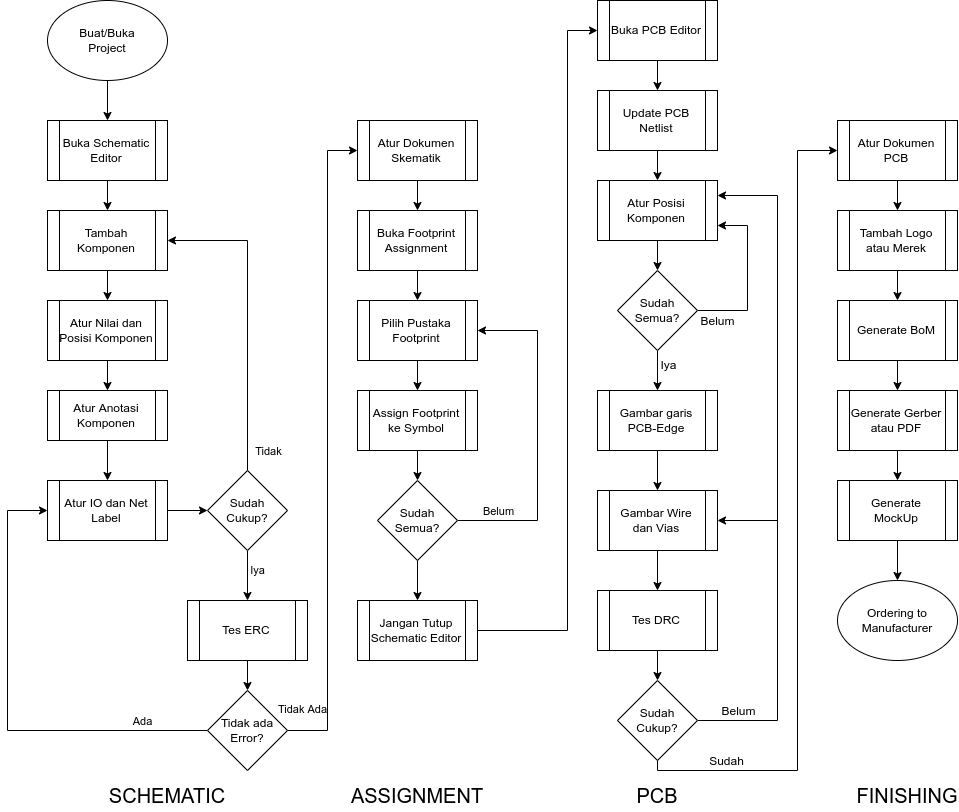
\includegraphics[width=\textwidth]{images/main/kicad_workflow}
		\caption{Workflow Umum KiCAD}
	\end{figure}

	\textbf{TIPS:} Tidak perlu menghafal secara fix untuk proses diagram di atas, cukup dijadikan sebagai panduan umum.

	\newpage
	\section{Project Baru}

	Untuk membuat project kosong baru, klik icon \menu{Create New Blank Project} seperti digambar ini:

	\begin{figure}[!ht]
		\centering
		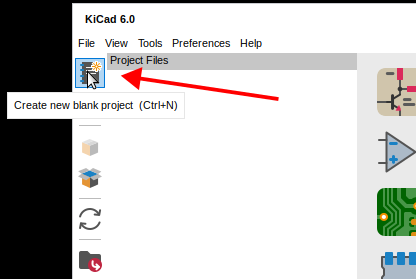
\includegraphics[width=0.4\textwidth]{images/main/kicad_new_0}
		\caption{Project Baru}
	\end{figure}

	Pilih folder dan beri nama project tersebut. Contoh disini adalah \textbf{esp32relay}.

	\begin{figure}[!ht]
		\centering
		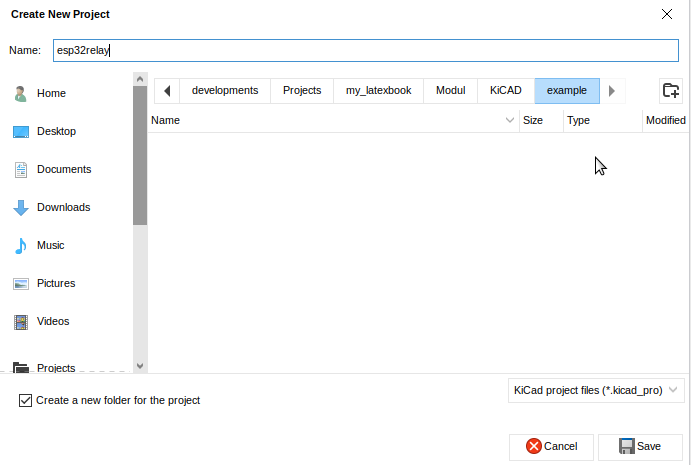
\includegraphics[width=0.5\textwidth]{images/main/kicad_new_1}
		\caption{Nama Project}
	\end{figure}

	Kemudian akan menghasilkan 3 berkas utama, yaitu \textbf{*.kicad\_pro} (berkas project),
	\textbf{*.kicad\_sch} (berkas skematik), dan \textbf{*.kicad\_pcb} (berkas PCB).

	\begin{figure}[!ht]
		\centering
		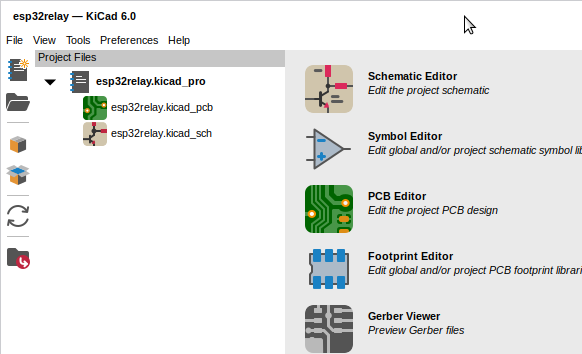
\includegraphics[width=0.6\textwidth]{images/main/kicad_new_2}
		\caption{Berkas Project}
	\end{figure}

	%%%%%%%%%%%%%%%%%%%%%%%%%%%%%%%%%%%%%%%%%%%%%%%%%%%%%%%%%%%%%%%%%

	\newpage
	\chapter{Schematic}
	Schematic adalah dokumen rancang sirkuit elektronik yang berisi simbol komponen beserta jaringan sinyal pinout atau catu daya.

	\section{Schematic Editor}

	Program Schematic Editor dapat dijalankan melalui program utama KiCAD:

	\begin{figure}[!ht]
		\centering
		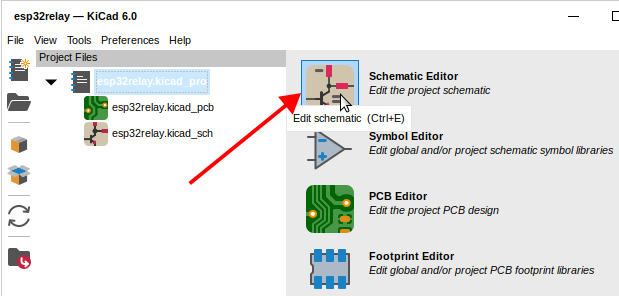
\includegraphics[width=0.6\textwidth]{images/sch/sch_0}
		\caption{Memanggil editor skematik}
	\end{figure}

	Jika baru pertama kali dijalankan akan ada konfirmasi pengaturan sumber pustaka symbol.
	Pilih saja yang direkomendasikan dan klik \menu{OK}.

	\begin{figure}[!ht]
		\centering
		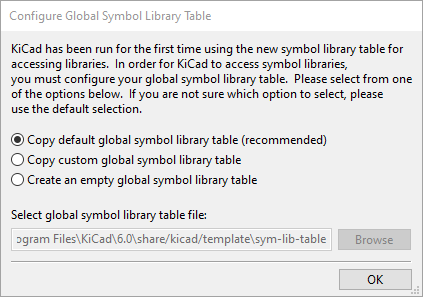
\includegraphics[width=0.5\textwidth]{images/installations/kicad_first_sch}
		\caption{Pilihan sumber pustaka}
	\end{figure}

	\newpage
	Berikut tampilan awal Schematic Editor
	\begin{figure}[!ht]
		\centering
		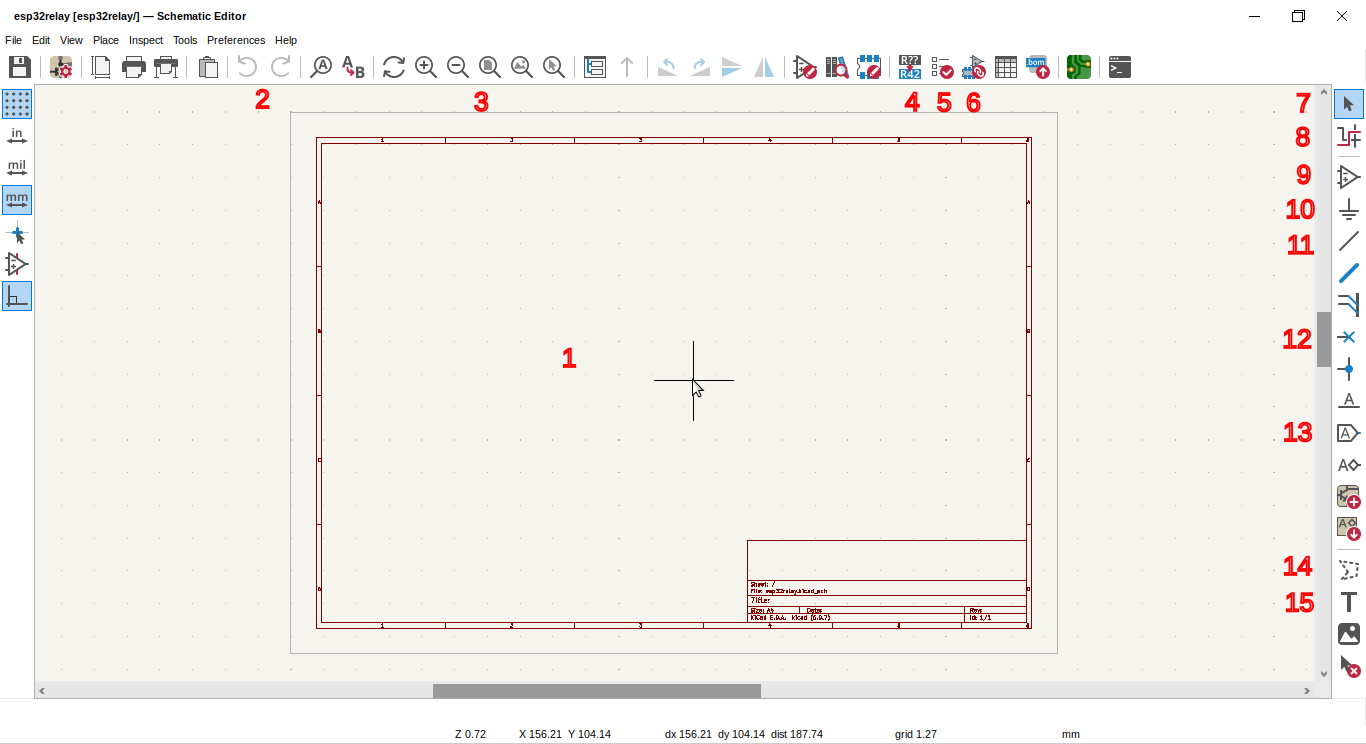
\includegraphics[width=\textwidth]{images/sch/sch_1}
		\caption{Schematic Editor}
	\end{figure}

	Penjelasan singkat tiap bagian:
	\begin{enumerate}[label=\textbf{\arabic*}.]
		\item Kanvas untuk menggambar skematik
		\item Toolbar perintah Undo-Redo
		\item Toolbar pengaturan tampilan skematik
		\item Toolbar perintah Anotasi komponen
		\item Toolbar perintah test ERC
		\item Toolbar perintah untuk Footprint Assignment
		\item Mode pointer default (dapat juga dengan menekan \keys{esc} pada keyboard)
		\item Mode tracking jalur baik di skematik maupun PCB
		\item Mode menambahkan komponen
		\item Mode menambahkan jaringan catu daya
		\item Mode menambahkan wiring
		\item Mode penanda Not-Connected
		\item Mode label sinyal
	\end{enumerate}

	\textbf{PERHATIAN:} Panduan selanjutnya akan menggunakan angka-angka di atas sebagai acuan (\textbf{Sch:X}).\\

	\textbf{TIPS:} Untuk memanipulasi objek di skematik maupun PCB, dapat melalui klik kanan objek yang ingin dimanipulasi.
	Sementara klik kanan pada area kosong dapat digunakan untuk menggeser kanvas.

	\newpage
	\section{Rancang Skematik}

	\subsection{Komponen ESP32}

	Selanjutnya untuk menambahkan komponen, kita dapat klik menu \menu[,]{Place, Add Symbol}, atau klik \textbf{Sch:9}.
	Akan muncul dialog database komponen, cari dengan term \textbf{esp32}.

	Pilih komponen ESP32-WROOM-32, pada dialog akan tampil pratinjau symbol dan default footprint yang tersedia.
	\begin{figure}[!ht]
		\centering
		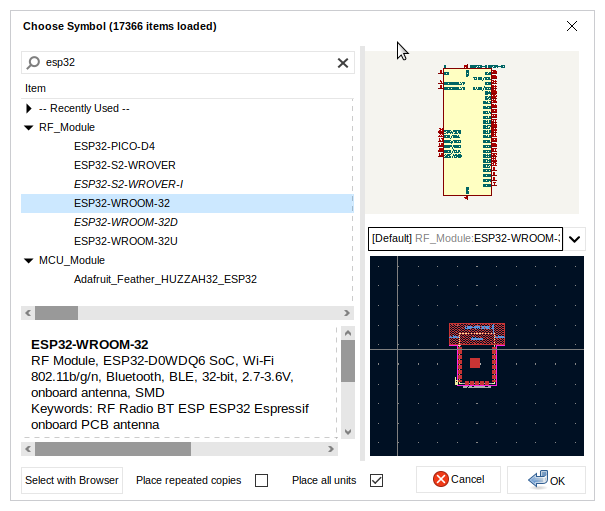
\includegraphics[width=0.6\textwidth]{images/sch/sch_2}
		\caption{Dialog Komponen}
	\end{figure}

	Untuk memulai penempatan komponen, klik \menu{OK}

	\begin{figure}[!ht]
		\centering
		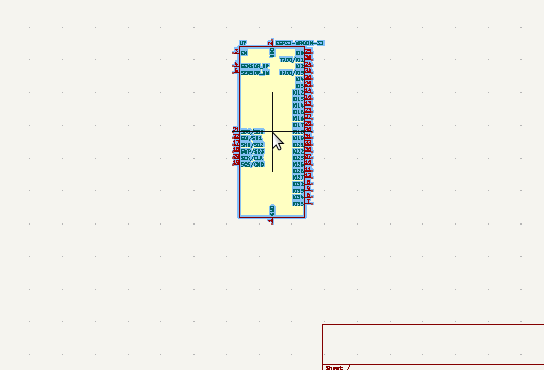
\includegraphics[width=0.55\textwidth]{images/sch/sch_3}
		\caption{Penempatan ESP32}
	\end{figure}

	Geser mouse ke tempat yang anda anggap cocok, tekan klik kiri untuk menempatkan.
	Anda juga dapat melakukan zoom-in dan zoom-out menggunakan roda mouse.

	Jika setelah menempatkan komponen kembali muncul dialog database komponen, silahkan tekan \menu{Cancel}
	dan kembali ke mode mouse pointer default (tekan \keys{esc} pada keyboard).

	\newpage
	\subsection{Penambahan Sinyal}

	Selanjutnya kita melakukan penambahan jaringan sinyal ke komponen ESP32.
	Sebagai contoh pertama kita tambahkan sinyal TX0 (transmitter untuk UART).
	Klik \menu[,]{Place,Add Global Label} atau klik \textbf{Sch:13}.

	\begin{figure}[!ht]
		\centering
		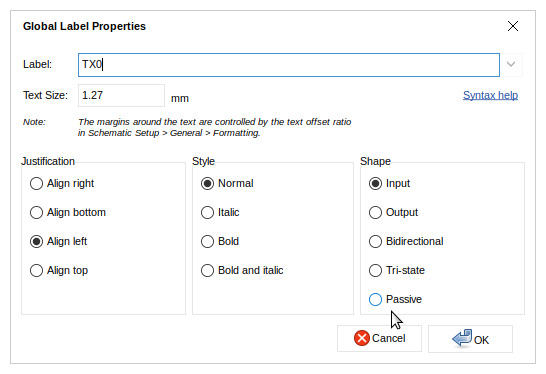
\includegraphics[width=0.5\textwidth]{images/sch/sch_4}
		\caption{Sinyal Properties}
	\end{figure}

	Isi nama sinyal dengan \textbf{TX0} dan klik \menu{OK}.
	Kemudian tempatkan label sinyal pada IO1 dengan pangkal-lingkar bertemu pangkal-lingkar seperti di bawah ini:

	\begin{figure}[!ht]
		\centering
		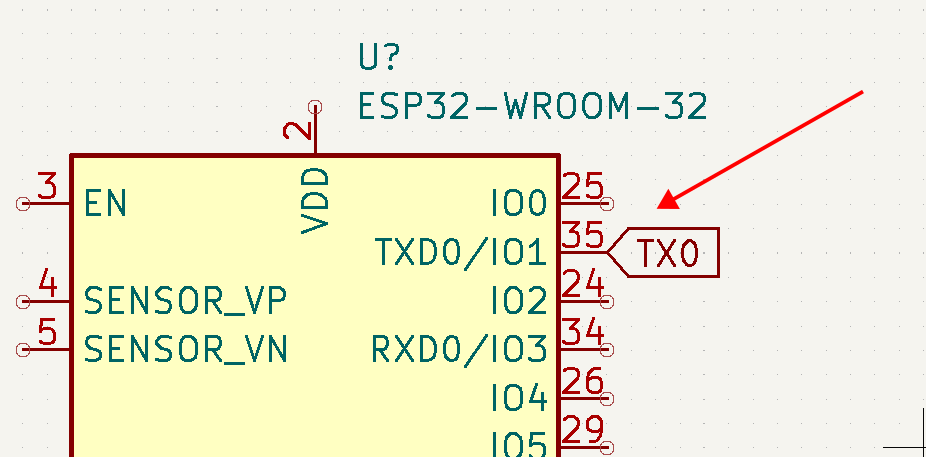
\includegraphics[width=0.5\textwidth]{images/sch/sch_5}
		\caption{Sinyal TX0}
	\end{figure}

	Kemudian dengan cara serupa, tempatkan sinyal \textbf{RX0} ke IO3

	\begin{figure}[!ht]
		\centering
		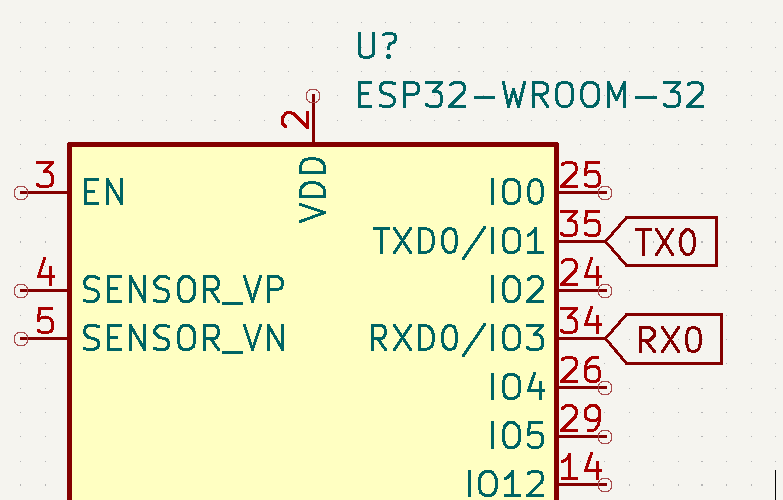
\includegraphics[width=0.5\textwidth]{images/sch/sch_6}
		\caption{Sinyal RX0}
	\end{figure}

	\newpage
	Lanjutkan penambahan sinyal mengikuti tabel berikut:

	\begin{table}[h!]
		\begin{center}
			\begin{tabular}{|l|l|l|l|l|l|}
				\toprule
				Sinyal & IO & Sinyal & IO & Sinyal & IO \\
				\midrule
				TX0 & IO1 & RX0 & IO3 & LED & IO2 \\
				FLASH & IO0 & RESET & EN & - & - \\
				ADC2\_CH4 & IO13 & ADC2\_CH6 & IO14 & - & - \\
				\bottomrule
			\end{tabular}
			\caption{ESP32 Sinyal IO}
		\end{center}
	\end{table}

	\begin{figure}[!ht]
		\centering
		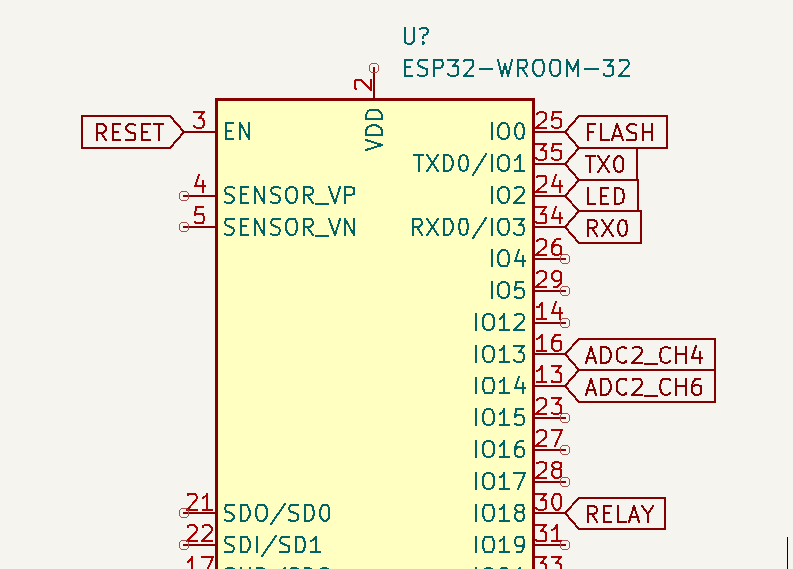
\includegraphics[width=0.5\textwidth]{images/sch/sch_7}
		\caption{Sinyal Utama}
	\end{figure}

	\textbf{TIPS:} Untuk manipulasi objek di skematik, selain menggunakan klik kanan, dapat pula menggunakan
	keyboard shortcut:
	\begin{itemize}
		\item \textbf{m}. Move atau memindahkan objek.

		\item \textbf{r}. Rotate atau memutar objek.

		\item \textbf{f}. Flip atau menukar orientasi objek.
	\end{itemize}

	Untuk objek \textbf{Global Label}, memanipulasi tanpa menekan shortcut di atas akan mengubah posisi objek namun wiring tetap tersambung.

	\subsection{Penambahan Jalur Daya}

	Jalur daya akan ditambahkan disini adalah \textbf{VDD} (3.3v) dan acuan \textbf{GND} (0v).
	Klik menu \menu[,]{Place,Add Power} atau kli \textbf{Sch:10}.

	\begin{figure}[!ht]
		\centering
		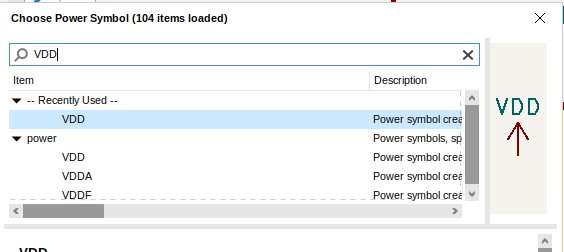
\includegraphics[width=0.4\textwidth]{images/sch/sch_8}
		\caption{Dialog Catu Daya}
	\end{figure}

	\textbf{TIPS:} Secara mendasar, jalur catu daya dapat diperlakukan sebagaimana layaknya komponen

	\begin{figure}[!ht]
		\centering
		\begin{subfigure}[t]{0.1\textwidth}
			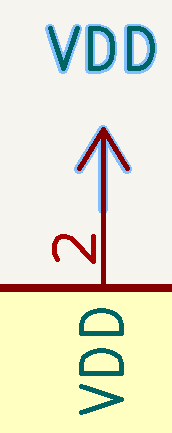
\includegraphics[width=\textwidth]{images/sch/sch_vdd}
			\caption{VDD}
		\end{subfigure}
		\begin{subfigure}[t]{0.1\textwidth}
			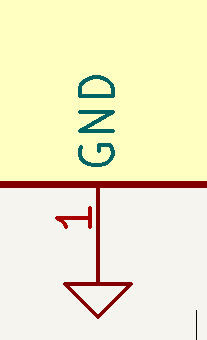
\includegraphics[width=\textwidth]{images/sch/sch_gnd}
			\caption{GND}
		\end{subfigure}
		\caption{Jalur catu daya}
	\end{figure}

	\subsection{Resistor Pull Down}

	Pada ESP32, jalur IO5 dan IO12 perlu ditarik ke level GND untuk memastikan booting chip.
	Untuk itu perlu ditambahkan resistor 0 ohm yang menghubungkan IO tersebut ke GND.

	Untuk menambahkan Resistor, kembali ke menu \menu[,]{Place,Add Symbol} atau klik \textbf{Sch:9}.
	Masukkan \textbf{R} ke kolom search.

	\begin{figure}[!ht]
		\centering
		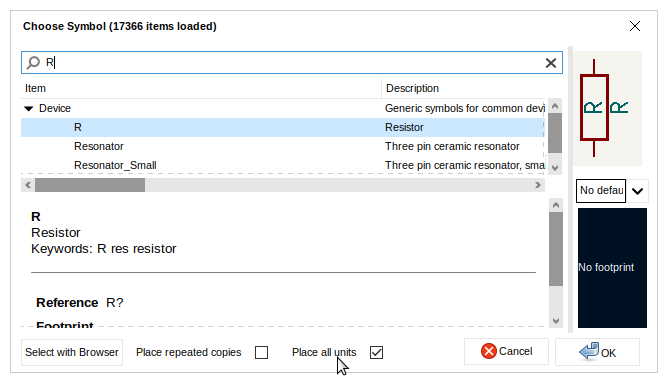
\includegraphics[width=0.55\textwidth]{images/sch/sch_9}
		\caption{Resistor}
	\end{figure}

	\textbf{PERHATIAN:} Resistor hanya memiliki default symbol, namun untuk footprint akan
	ditentukan nanti saat Assignment.\\

	Tempatkan Resistor dekat IO5 seperti berikut ini:
	\begin{figure}[!ht]
		\centering
		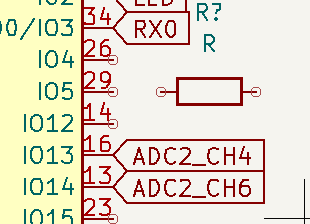
\includegraphics[width=0.4\textwidth]{images/sch/sch_10}
		\caption{Resistor IO5}
	\end{figure}

	Untuk memodifikasi nilai, double-klik huruf R yang tidak ada simbol (?) di dekatnya.
	\begin{figure}[!ht]
		\centering
		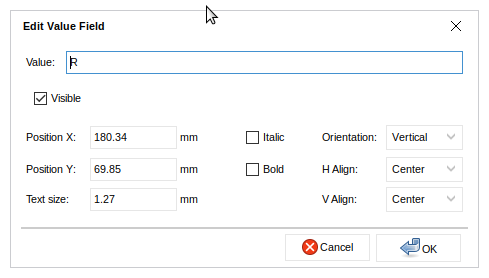
\includegraphics[width=0.55\textwidth]{images/sch/sch_11}
		\caption{Ganti Nilai}
	\end{figure}

	Ganti huruf \textbf{R} menjadi angka \textbf{0}. Kemudian klik \menu{OK}.

	\begin{figure}[!ht]
		\centering
		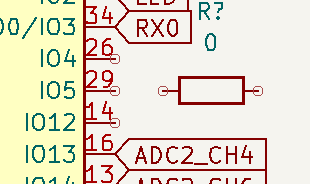
\includegraphics[width=0.55\textwidth]{images/sch/sch_12}
		\caption{Resistor 0 untuk IO5}
	\end{figure}

	Duplikat resistor tersebut dengan klik kanan dan klik \menu{Duplicate}
	atau langsung tekan \keys[,]{ctrl,d} di keyboard.
	Taruh komponen duplikat dekat IO12.\\

	\textbf{TIPS:} Anda dapat pula menggeser nilai dan nama komponen agar terlihat lebih jelas.

	\begin{figure}[!ht]
		\centering
		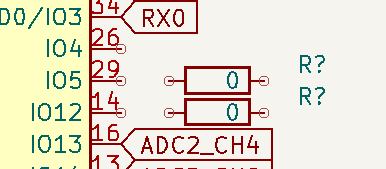
\includegraphics[width=0.55\textwidth]{images/sch/sch_13}
		\caption{Resistor 0 untuk booting}
	\end{figure}

	Selanjutnya ambil satu GND dan letakkan dekat kedua komponen tersebut.

	\newpage
	Kemudian karena komponen berdekatan, dapat dipilih menghubungkan pangkal-lingkar komponen
	menggunakan wiring.
	Klik menu \menu[,]{Place,Add Wire} atau klik \textbf{Sch:11}.\\

	Taruh pointer mouse ke salah satu pangkal-lingkar, klik kiri,
	kemudian geser ke pangkal-lingkar lain yang akan dihubungkan, kemudian klik kiri sekali lagi.\\

	Hubungkan wire hingga seperti ini:

	\begin{figure}[!ht]
		\centering
		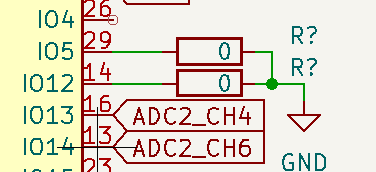
\includegraphics[width=0.5\textwidth]{images/sch/sch_14}
		\caption{Wire untuk untuk booting}
	\end{figure}

	\subsection{Menambahkan Anotasi}

	Proses Anotasi adalah mengubah simbol (?) menjadi angka yang dapat menjadi index pembeda antara
	satu komponen dengan komponen lain yang sejenis.
	Untuk melakukan Anotasi, klik menu \menu[,]{Tools,Annotate Schematic} atau klik \textbf{Sch:4}.
	Kemudian klik \menu{Annotate} dan \menu{Close} saat selesai.

	\begin{figure}[!ht]
		\centering
		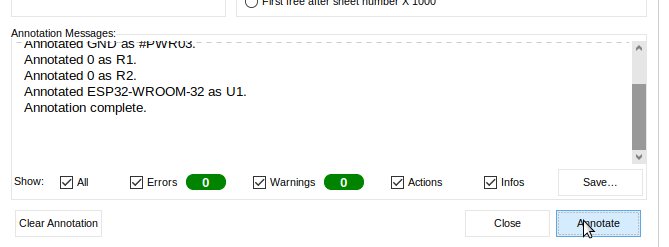
\includegraphics[width=0.6\textwidth]{images/sch/sch_15}
		\caption{Dialog Annotasi}
	\end{figure}

	Simbol (?) disebelah nama komponen yang telah tergantikan dengan angka yang berbeda di tiap project.

	\begin{figure}[!ht]
		\centering
		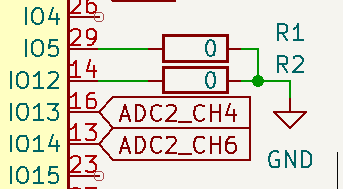
\includegraphics[width=0.5\textwidth]{images/sch/sch_16}
		\caption{Komponen telah teranotasi}
	\end{figure}

	\textbf{TIPS:} Anda dapat melakukan \menu{Save} (menu \menu[,]{File,Save} atau \keys[,]{ctrl,s}) dan \menu{Annotate Schematic} sesering yang anda suka.

	\newpage
	\subsection{Penanda Not-Connected}

	Agar tidak membingungkan proses tes ERC (Electrical Rule Check), maka pin ESP32 yang digunakan perlu ditandai sebagai Not-Connected.
	Klik menu \menu[,]{Place,Add No Connect Flag} atau klik \textbf{Sch:12}.\\

	Kemudian klik kiri tiap pangkal-lingkar dari pin ESP32 yang tidak tehubung kemanapun.

	\begin{figure}[!ht]
		\centering
		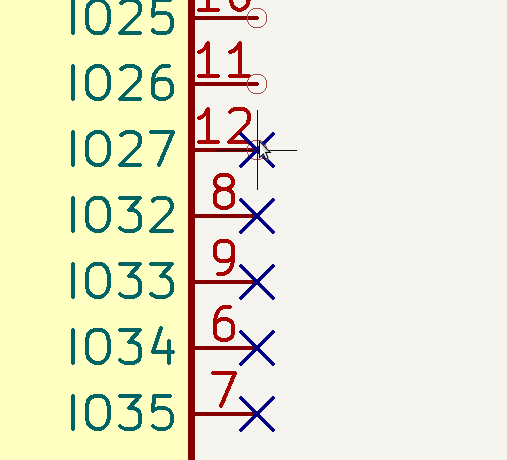
\includegraphics[width=0.4\textwidth]{images/sch/sch_17}
		\caption{Penanda Not-Connected}
	\end{figure}

	\subsection{Sisa Skematik Selanjutnya}

	Diharapkan sudah mampu menggambar secara mandiri.\\

	\textbf{TIPS:} Global Label dapat juga dilakukan \menu{Duplicate} sebagaimana layaknya komponen.

	\subsubsection{Tombol Reset, Flash, Pin Programming}

	\begin{figure}[!ht]
		\centering
		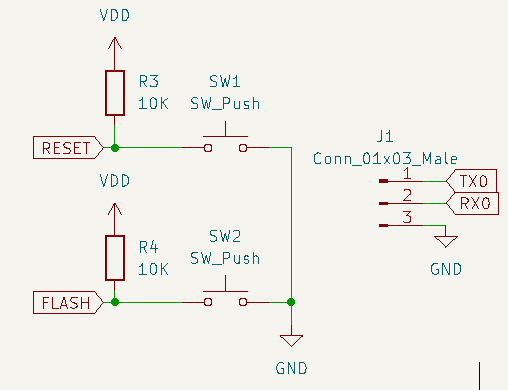
\includegraphics[width=0.5\textwidth]{images/sch/sch_18}
		\caption{Reset, Flash dan Header Programming}
	\end{figure}

	\newpage
	\subsubsection{LED dan Decouple-Capacitor}

	\begin{figure}[!ht]
		\centering
		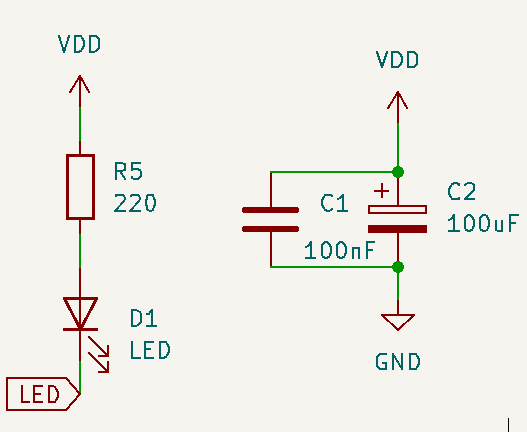
\includegraphics[width=0.4\textwidth]{images/sch/sch_19}
		\caption{LED dan Decouple}
	\end{figure}

	\subsubsection{Sensor dan Referensi}

	\begin{figure}[!ht]
		\centering
		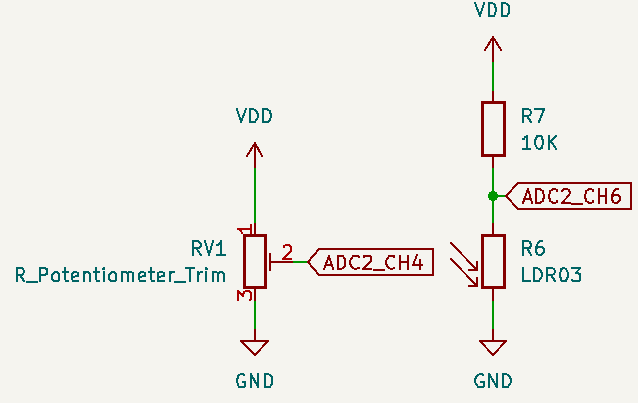
\includegraphics[width=0.4\textwidth]{images/sch/sch_20}
		\caption{Sensor dan Pengaturan Referensi}
	\end{figure}

	\subsubsection{Voltage Regulator dan Lubang-Baut}

	\begin{figure}[!ht]
		\centering
		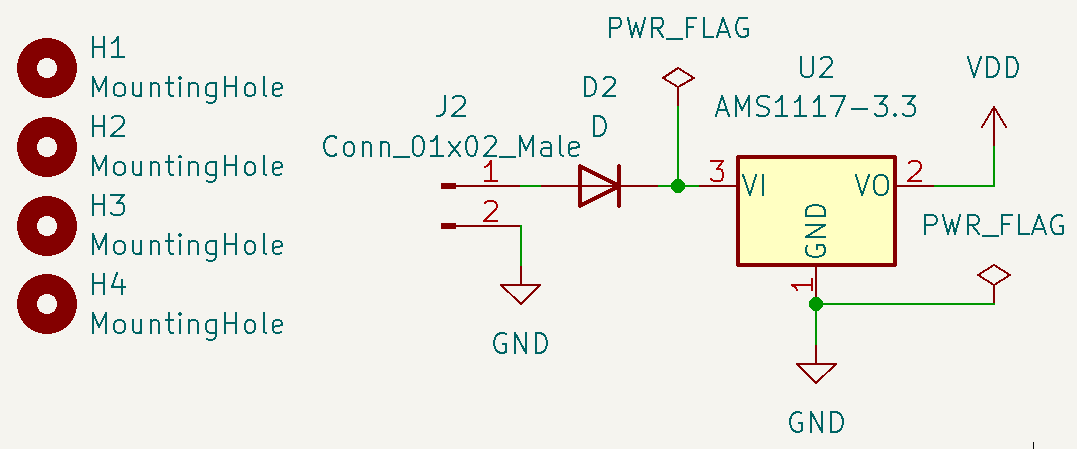
\includegraphics[width=0.6\textwidth]{images/sch/sch_21}
		\caption{Voltage Regulator dan Lubang-Baut}
	\end{figure}

	\textbf{PERHATIAN:} Jangan lupa menambahkan penanda \textbf{PWR\_FLAG} yang tersedia di
	jalur catu daya agar tes ERC valid.
	Label \textbf{PWR\_FLAG} tersedia di menu \menu[,]{Place,Add Power} atau \textbf{Sch:10}.

	\newpage
	\subsection{Atur Dokumen}
	Langkah selanjutnya anda dapat mengatur properti dokumen.
	Klik menu \menu[,]{File,Page Settings}.
	Akan muncul dialog berikut.
	Klik \menu{OK} setelah pengaturan dianggap cukup.

	\begin{figure}[!ht]
		\centering
		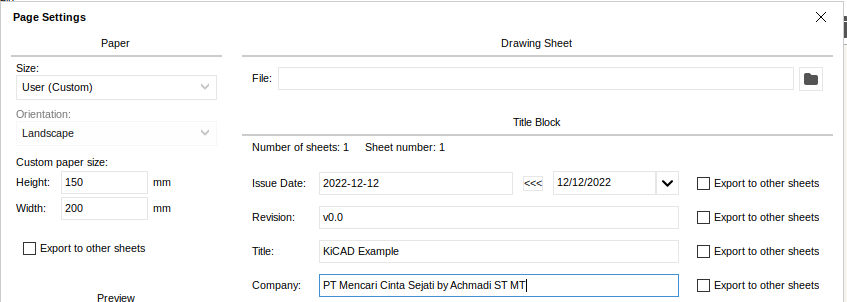
\includegraphics[width=0.8\textwidth]{images/sch/sch_set}
		\caption{Setting Dokumen}
	\end{figure}

	\section{Tes ERC}

	Untuk cek skematik, dapat memanfaatkan fitur ERC yang tersedia di menu \menu[,]{Inspect, Electrical Rules Checker} atau \textbf{Sch:5}.
	Kemudian klik \menu{Run ERC} dan tunggu hingga cek selesai:
	\begin{figure}[!ht]
		\centering
		\begin{subfigure}[t]{0.45\textwidth}
			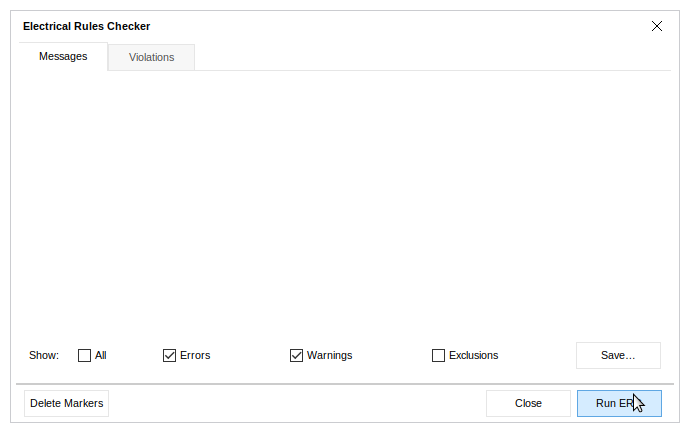
\includegraphics[width=\textwidth]{images/sch/erc_0}
			\caption{Mulai}
		\end{subfigure}
		\begin{subfigure}[t]{0.45\textwidth}
			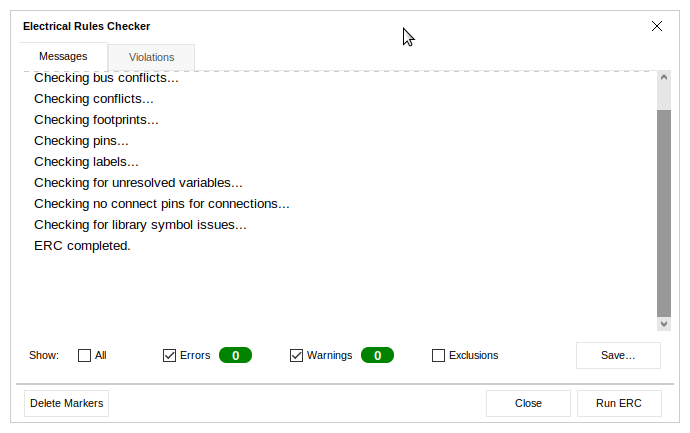
\includegraphics[width=\textwidth]{images/sch/erc_1}
			\caption{Sukses}
		\end{subfigure}
		\caption{tes ERC}
	\end{figure}

	\begin{figure}[!ht]
		\centering
		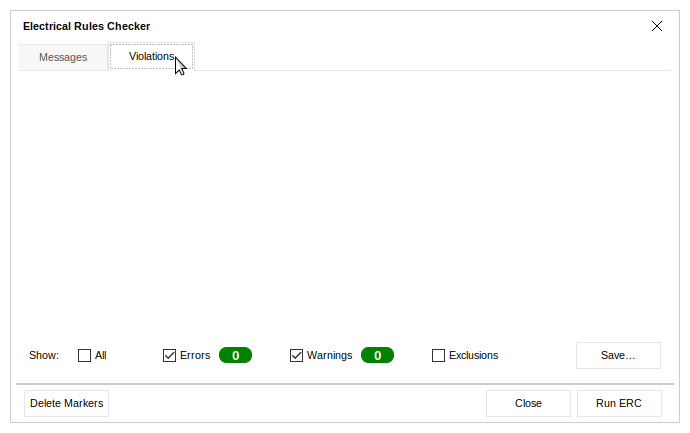
\includegraphics[width=0.45\textwidth]{images/sch/erc_2}
		\caption{Pastikan Violation kosong}
	\end{figure}

	\newpage
	\section{Skematik Penuh}

	\begin{figure}[!ht]
		\centering
		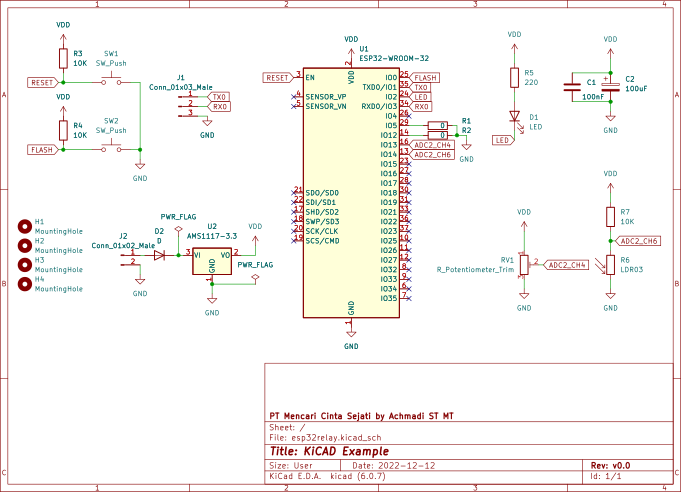
\includegraphics[width=\textwidth]{images/sch/esp32relay}
		\caption{Skematik Penuh}
	\end{figure}

	\begin{center}
		\textbf{Sampai disini, rancang skematik telah selesai.}
	\end{center}

	%%%%%%%%%%%%%%%%%%%%%%%%%%%%%%%%%%%%%%%%%%%%%%%%%%%%%%%%%%%%%%%%%

	\newpage
	\chapter{Footprint Assignment}

	Footprint Assignment adalah proses menautkan antara symbol pada skematik dengan footprint (representasi nyata komponen)
	yang nantinya akan digunakan pada layout PCB.
	Satu symbol seperti resistor misalnya dapat memiliki beberapa pilihan footprint.

	\section{FP Assign}
	Program untuk footprint assignment dapat dijalankan dari Schematic Editor melalui
	menu \menu[,]{Tools,Assign Footprints} atau klik \textbf{Sch:6}.
	Berikut tampilan awal Footprint Assigment
	\begin{figure}[!ht]
		\centering
		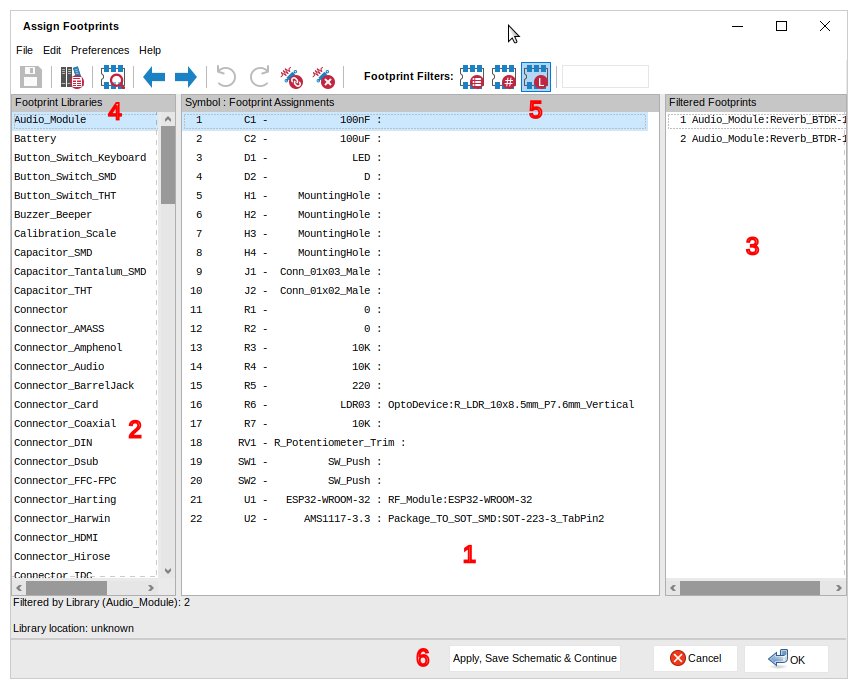
\includegraphics[width=0.8\textwidth]{images/fpa/fpa_1}
		\caption{Footprint Assigment}
	\end{figure}

	Penjelasan singkat tiap bagian:
	\begin{enumerate}[label=\textbf{\arabic*}.]
		\item Kolom daftar footprint assigment
		\item Kolom daftar pustaka footprint yang tersedia
		\item Kolom daftar footprint yang dapat dipilih
		\item Toolbar untuk pratinjau model footprint
		\item Toolbar untuk pilih mode seleksi pustaka
		\item Tombol untuk simpan dan menyelesaikan.
	\end{enumerate}

	\textbf{PERHATIAN:} Panduan selanjutnya akan menggunakan angka-angka di atas sebagai acuan (\textbf{Fpa:X}).\\

	\textbf{TIPS:} Anda dapat klik \menu{Apply, Save Schematic and Continue} sesering yang anda suka.\\

	\textbf{TIPS:} Disarankan menggunakan mode seleksi footprint \textbf{Fpa:5} berdasarkan library (L) agar terkumpul sesuai pustaka.\\

	\textbf{TIPS:} Klik \menu{Apply, Save Schematic and Continue} tidak menutup dialog footprint assigment.
	Klik \menu{Cancel} atau \menu{OK} untuk menutup dialog tersebut.\\

	\section{Langkah Assignment}

	Berikut urutan langkah footprint assignment secara umum.
	Disini dipilih resistor sebagai contoh pertama.

	\begin{enumerate}
		\item Pilih komponen atau kelompok komponen di kolom \textbf{Fpa:1}.
		Dapat digunakan tombol \keys{shift} dan panah atas-bawah untuk memilih beberapa komponen.

		\begin{figure}[!ht]
			\centering
			\includegraphics[width=0.8\textwidth]{images/fpa/fpa_2}
			\caption{Pilih komponen}
		\end{figure}

		\newpage
		\item Pilih pustaka \textbf{Resistor SMD} di kolom \textbf{Fpa:2}.

		\begin{figure}[!ht]
			\centering
			\includegraphics[width=0.8\textwidth]{images/fpa/fpa_3}
			\caption{Pilih Pustaka}
		\end{figure}

		Dapat terlihat kolom pilihan footprint \textbf{Fpa:3} sudah berubah menyesuaikan pilihan pustaka.

		\item Pilih footprint yang sesuai dan tersedia di pembelian nantinya.
		Sebagai contoh disini dipilih Resistor SMD tipe 0805

		\begin{figure}[!ht]
			\centering
			\includegraphics[width=0.8\textwidth]{images/fpa/fpa_4}
			\caption{Pilih Footprint}
		\end{figure}

		\textbf{TIPS:} Nama footprint pada dialog assigment berpola \textbf{Pustaka:Footprint\_Variasi}.

		\newpage
		\item Anda dapat pula pratinjau model footprint yang tersedia dengan klik \textbf{Fpa:4}

		\begin{figure}[!ht]
			\centering
			\includegraphics[width=0.6\textwidth]{images/fpa/fpa_5}
			\caption{Model Footprint}
		\end{figure}

		Tutup jendela pratinjau jika dianggap sudah sesuai.

		\item Kemudian double-click footprint yang dipilih di kolom \textbf{Fpa:3}.
		Komponen yang dipilih akan diset sesuai footprint yang di double-click.

		\begin{figure}[!ht]
			\centering
			\includegraphics[width=0.8\textwidth]{images/fpa/fpa_6}
			\caption{Footprint Assigment untuk Resistor}
		\end{figure}

		Klik \menu{Apply, Save Schematic and Continue} dan lanjutkan ke komponen lainnya
		yang belum memiliki footprint.

	\end{enumerate}

	\textbf{TIPS:} Dapat pula dicek model 3D komponen dengan klik icon komponen 3D pada jendela pratinjau footprint.

	\newpage
	\begin{figure}[!ht]
		\centering
		\begin{subfigure}[t]{0.45\textwidth}
			\includegraphics[width=\textwidth]{images/fpa/fpa_7}
			\caption{Pratinjau 3D}
		\end{subfigure}
		\begin{subfigure}[t]{0.45\textwidth}
			\includegraphics[width=\textwidth]{images/fpa/fpa_8}
			\caption{Model 3D}
		\end{subfigure}
		\caption{3D Footprint}
	\end{figure}

	\newpage
	\section{Footprint Assigment Penuh}

	Berikut contoh Footprint Assigment secara penuh:

	\begin{figure}[!ht]
		\centering
		\includegraphics[width=\textwidth]{images/fpa/fpa_full}
		\caption{Contoh Footprint Assigment}
	\end{figure}

	\begin{center}
		\textbf{Sampai disini, footprint assigment telah selesai.}
	\end{center}

	%%%%%%%%%%%%%%%%%%%%%%%%%%%%%%%%%%%%%%%%%%%%%%%%%%%%%%%%%%%%%%%%%

	\newpage
	\chapter{PCB Layout}

	PCB Layout adalah dokumen rancang sirkuit sebenarnya yang berisi representasi kompenen
	yang menjadi penyusun unit PCB.
	Jaringan dan komponen PCB Layout dibuat berdasarkan dokumen Schematic.

	\section{PCB Editor}

	Program PCB Editor dapat dijalankan melalui program utama KiCAD:

	\begin{figure}[!ht]
		\centering
		\includegraphics[width=0.6\textwidth]{images/pcb/pcb_0}
		\caption{Memanggil editor pcb}
	\end{figure}

	Jika baru pertama kali dijalankan akan ada konfirmasi pengaturan sumber pustaka footprint.
	Pilih saja yang direkomendasikan dan klik \menu{OK}.

	\begin{figure}[!ht]
		\centering
		\includegraphics[width=0.5\textwidth]{images/installations/kicad_first_pcb}
		\caption{Pilihan sumber pustaka}
	\end{figure}

	\newpage
	Berikut tampilan awal PCB Editor
	\begin{figure}[!ht]
		\centering
		\includegraphics[width=\textwidth]{images/pcb/pcb_1}
		\caption{PCB Editor}
	\end{figure}

	Penjelasan singkat tiap bagian:
	\begin{enumerate}[label=\textbf{\arabic*}.]
		\item Kanvas untuk menggambar PCB
		\item Toolbar perintah Undo-Redo
		\item Toolbar pengaturan tampilan skematik
		\item Dropdown pilihan lebar jalur
		\item Toolbar update PCB dari skematik
		\item Toolbar perintah tes DRC
		\item Dropdown pilihan layer yang aktif
		\item Mode pointer default (dapat juga dengan menekan \keys{esc} pada keyboard)
		\item Mode menambahkan wire
		\item Mode menambahkan fill-area
		\item Mode menambahkan shape
		\item Mode menambahkan teks
		\item Kolom Layer Manager
	\end{enumerate}

	\textbf{PERHATIAN:} Panduan selanjutnya akan menggunakan angka-angka di atas sebagai acuan (\textbf{Pcb:X}).\\

	\textbf{TIPS:} Untuk memanipulasi objek di skematik maupun PCB, dapat melalui klik kanan objek yang ingin dimanipulasi.
	Sementara klik kanan pada area kosong dapat digunakan untuk menggeser kanvas.

	\newpage
	\section{Rancang PCB}

	\subsection{Pengaturan Desain}

	Berikut beberapa pengaturan dasar desain yang direkomendasikan.
	Tahap ini hanya sekedar penyesuaian dengan vendor pemesanan PCB lokal yang pernah penulis pesan.
	Untuk membuka dialog pengaturan desain, klik menu \menu[,]{File,Board Setup}

	Beberapa pengaturan yang biasa penulis gunakan:
	\begin{itemize}
		\item Buka \menu[,]{Text and Graphics,Defaults}, isi nilai \textbf{Edge Cuts} sebesar 0.5mm

		\begin{figure}[!ht]
			\centering
			\includegraphics[width=0.6\textwidth]{images/pcb/pcb_set_0}
			\caption{Pengaturan Edge-Cuts}
		\end{figure}

		\item Buka \menu[,]{Design Rules,Pre-defined Sizes}, tambahkan pilihan lebar wire pada kolom \menu{Tracks}.
		Klik icon \menu{+} di bawah kolom untuk menambahkan.

		\begin{figure}[!ht]
			\centering
			\includegraphics[width=0.6\textwidth]{images/pcb/pcb_set_1}
			\caption{Pengaturan Pilihan Lebar Wire}
		\end{figure}

		\item Buka \menu[,]{Design Rules,Net Classes}, ganti ukuran \textbf{Via Size} ke \textbf{1.4 mm}
		dan \textbf{Via Hole} menjadi \textbf{0.7 mm}.

		\begin{figure}[!ht]
			\centering
			\includegraphics[width=0.6\textwidth]{images/pcb/pcb_set_2}
			\caption{Pengaturan default Net Class}
		\end{figure}
	\end{itemize}

	Setelah selesai, Klik \menu{OK}.

	\newpage
	Kemudian dropdown pilihan lebar wire akan menampilkan pilihan yang tadi dibuat.
	Untuk ukuran \textbf{Grid}, disarankan ambil \textbf{0.01 mm} saja.
	Simpan berkas dengan shortcut \keys[,]{ctrl,s} atau melalui menu \menu[,]{File,Save}.

	\begin{figure}[!ht]
		\centering
		\includegraphics[width=0.7\textwidth]{images/pcb/pcb_set_3}
		\caption{Pengaturan Design selesai}
	\end{figure}

	\subsection{Update PCB dari Schematic}

	Jika Schematic telah siap dan selesai footprint assigment, maka dapat dilakukan impor desain ke PCB.
	Klik menu \menu[,]{Tools,Update PCB from Schematic} atau klik \textbf{Pcb:5}.
	Akan muncul dialog seperti ini:

	\begin{figure}[!ht]
		\centering
		\includegraphics[width=0.65\textwidth]{images/pcb/pcb_2}
		\caption{Dialog update PCB}
	\end{figure}

	Jika tidak ada error atau warning, klik \menu{Update PCB} dan \menu{Close}.\\

	\textbf{TIPS:} Update PCB dapat dilakukan setiap ada modifikasi schematic atau footprint assignment.

	\newpage
	Setelah dialog update PCB ditutup, cursor akan mendapatkan grup komponen yang dapat ditaruh di kanvas.
	Taruh semua komponen di kanvas di luar area border.

	\begin{figure}[!ht]
		\centering
		\includegraphics[width=0.7\textwidth]{images/pcb/pcb_3}
		\caption{Komponen}
	\end{figure}

	\subsection{Peletakan Komponen}

	Langkah selanjutnya adalah peletakan setiap komponen.
	Sebagai contoh awal disini, dipilih komponen \textbf{ESP32}.
	Klik kiri komponen tersebut, geser ke dalam border, kemudian klik kiri kembali.

	\begin{figure}[!ht]
		\centering
		\includegraphics[width=0.6\textwidth]{images/pcb/pcb_4}
		\caption{Komponen ESP32}
	\end{figure}

	\textbf{TIPS:} Untuk manipulasi objek di pcb, selain menggunakan klik kanan, dapat pula menggunakan
	keyboard shortcut:
	\begin{itemize}
		\item \textbf{m}. Move atau memindahkan objek.

		\item \textbf{r}. Rotate atau memutar objek.

		\item \textbf{f}. Flip atau menukar layer objek dari top ke bottom atau sebaliknya.
	\end{itemize}

	\newpage
	Selanjutnya, diletakkan komponen resistor \textbf{R1} dan \textbf{R2} dekat \textbf{ESP32} pada IO5 dan IO12.\\

	\textbf{TIPS:} Dapat digunakan fasilitas pencarian yang ada di menu \menu[,]{Edit,Find} atau keyboard \keys[,]{ctrl,f}

	\begin{figure}[!ht]
		\centering
		\includegraphics[width=0.6\textwidth]{images/pcb/pcb_5}
		\caption{Komponen R1 dan R2}
	\end{figure}

	Lanjutkan ke decouple capacitor \textbf{C1} dan \textbf{C2}.

	\begin{figure}[!ht]
		\centering
		\includegraphics[width=0.6\textwidth]{images/pcb/pcb_6}
		\caption{Komponen C1 dan C2}
	\end{figure}

	\textbf{TIPS:} Gunakan Window Size Cursor dan Penggaris (tersedia di menu \menu[,]{Inspect,Measure Tool}) untuk mempermudah menentukan posisi komponen.

	\begin{figure}[!ht]
		\centering
		\begin{subfigure}[t]{0.2\textwidth}
			\includegraphics[width=\textwidth]{images/pcb/pcb_cursor}
			\caption{Window-Size Cursor}
		\end{subfigure}
		\begin{subfigure}[t]{0.45\textwidth}
			\includegraphics[width=\textwidth]{images/pcb/pcb_ruler}
			\caption{Penggaris}
		\end{subfigure}
		\caption{Alat Bantu}
	\end{figure}

	\newpage
	Lanjutkan penempatan komponen hingga seperti ini:

	\begin{figure}[!ht]
		\centering
		\includegraphics[width=0.8\textwidth]{images/pcb/pcb_7}
		\caption{PCB Penuh}
	\end{figure}

	\subsection{PCB Edge}

	Selanjutnya tambahkan PCB Edge dengan memilih \textbf{Edge.Cuts} pada dropdown pilihan layer (\textbf{Pcb:7}).
	Kemudian pilih gambar kotak dengan klik \textbf{Pcb:11}.

	\begin{figure}[!ht]
		\centering
		\begin{subfigure}[t]{0.35\textwidth}
			\includegraphics[width=\textwidth]{images/pcb/pcb_8}
			\caption{Layer Edge Cuts}
		\end{subfigure}
		\begin{subfigure}[t]{0.15\textwidth}
			\includegraphics[width=\textwidth]{images/pcb/pcb_9}
			\caption{Gambar Kotak}
		\end{subfigure}
		\caption{Gambar Edge Cuts}
	\end{figure}

	\newpage
	hasil kotak Edge Cuts:

	\begin{figure}[!ht]
		\centering
		\includegraphics[width=0.6\textwidth]{images/pcb/pcb_10}
		\caption{PCB dengan Edge Cuts}
	\end{figure}

	Kemudian melalui menu \menu[,]{View,3D Viewer}, dapat dilihat model mockup 3D dari PCB.

	\begin{figure}[!ht]
		\centering
		\includegraphics[width=0.8\textwidth]{images/pcb/pcb_11}
		\caption{Model 3D PCB}
	\end{figure}

	\textbf{TIPS:} Jika ada komponen tidak tampak model 3D, maka memang belum ada atau belum ditambahkan saja.\\

	\textbf{TIPS:} Model 3D komponen umumnya berformat \textbf{VRML} atau \textbf{STEP/STP} yang dapat dibuat sendiri atau didownload dari internet.

	\newpage
	\subsection{Track Route}

	Langkah penting selanjutnya adalah route track, untuk mengubah garis penanda koneksi (disebut Ratsnest)
	menjadi jalur tembaga sebenarnya.

	Berikut langkahnya:
	\begin{itemize}
		\item Pilih jalur \textbf{F.Cu} atau \textbf{B.Cu} di dropdown \textbf{Pcb:7}.

		\item Klik mode \textbf{Route Track} dengan klik \textbf{Pcb:9}.

		\item Pilih ukuran track di dropdown \textbf{Pcb:4}, semisal \textbf{0.5 mm}.

		\item Klik satu ruas garis Ratsnest, kemudian geser pointer untuk menggambar jalur,

		\item Klik kiri kembali untuk mengakhiri.
	\end{itemize}

	\begin{figure}[!ht]
		\centering
		\begin{subfigure}[t]{0.45\textwidth}
			\includegraphics[width=\textwidth]{images/pcb/pcb_12}
			\caption{Ratsnets}
		\end{subfigure}
		\begin{subfigure}[t]{0.45\textwidth}
			\includegraphics[width=\textwidth]{images/pcb/pcb_13}
			\caption{Routing}
		\end{subfigure}
		\caption{Track Route}
	\end{figure}

	\begin{figure}[!ht]
		\centering
		\includegraphics[width=0.45\textwidth]{images/pcb/pcb_14}
		\caption{Routing selesai}
	\end{figure}

	\newpage
	\subsection{Tambah Vias}

	Vias adalah komponen tambahan yang menjadi jembatan antara layer top dan layer bottom
	pada track.

	Untuk menambahkan vias, berikut langkahnya:
	\begin{itemize}
		\item Track route sebagaimana sebelumnya.
		\item Klik kanan, klik menu \menu{Place Through Via}.
		\item Klik kiri untuk menempatkan Via.
		\item Lanjutkan track route di layer sebaliknya setelah vias.
		\item Klik kiri untuk mengakhiri.
	\end{itemize}

	\begin{figure}[!ht]
		\centering
		\begin{subfigure}[t]{0.45\textwidth}
			\includegraphics[width=\textwidth]{images/pcb/pcb_15}
			\caption{Mulai Route}
		\end{subfigure}
		\begin{subfigure}[t]{0.45\textwidth}
			\includegraphics[width=\textwidth]{images/pcb/pcb_16}
			\caption{Pilih Mode Vias}
		\end{subfigure}
		\caption{Route Vias}
	\end{figure}

	\begin{figure}[!ht]
		\centering
		\begin{subfigure}[t]{0.45\textwidth}
			\includegraphics[width=\textwidth]{images/pcb/pcb_17}
			\caption{Taruh Vias}
		\end{subfigure}
		\begin{subfigure}[t]{0.45\textwidth}
			\includegraphics[width=\textwidth]{images/pcb/pcb_18}
			\caption{Jalur ber-Vias}
		\end{subfigure}
		\caption{Vias Selesai}
	\end{figure}

	\textbf{TIPS:} Tidak ada aturan khusus untuk Vias dan Track Route, namun selayaknya:
	\begin{itemize}
		\item Dahulukan Track/Vias jalur sinyal baru kemudian jalur catu daya.
		\item Ukuran jalur Track/Vias disesuaikan arus dan pin komponen.
		\item Mayoritas komponen sedapatnya berada layer yang sama.
	\end{itemize}

	\newpage
	Lanjutkan track routing hingga seperti ini:

	\begin{figure}[!ht]
		\centering
		\begin{subfigure}[t]{0.45\textwidth}
			\includegraphics[width=\textwidth]{images/pcb/pcb_19}
			\caption{Top}
		\end{subfigure}
		\begin{subfigure}[t]{0.45\textwidth}
			\includegraphics[width=\textwidth]{images/pcb/pcb_20}
			\caption{Bottom}
		\end{subfigure}
		\caption{Hasil Routing}
	\end{figure}

	\subsection{Tambah Filled Zone}

	Filled Zone adalah area tembaga yang bentuknya berupa luasan. Filled Zone dapat terhubung
	ke suatu sinyal, VDD, GND, atau tidak terhubung sama sekali.

	Untuk menambahkan filled zone, berikut langkahnya:
	\begin{itemize}
		\item Klik menu \menu[,]{Place, Add Filled Zone}
		\item Klik kiri pojok kiri atas dari garis kotak EdgeCuts.
		Akan muncul dialog pengaturan filled zone.
		\item Pilih \textbf{no-net} sebagai jalur untuk kedua layer tembaga (\textbf{F.Cu }dan \textbf{B.Cu}).
		Pilihan lainnya biarkan default.

		\begin{figure}[!ht]
			\centering
			\includegraphics[width=0.65\textwidth]{images/pcb/pcb_21}
			\caption{Pengaturan Filled Zone}
		\end{figure}

		Klik \menu{OK} untuk melanjutkan.

		\newpage
		\item Klik kiri pada pojok kanan atas dari garis kotak EdgeCuts.
		\item Klik kiri pada pojok kanan bawah dari garis kotak EdgeCuts.
		\item Klik kiri pada pojok kiri bawah dari garis kotak EdgeCuts untuk mengakhiri.

		\begin{figure}[!ht]
			\centering
			\begin{subfigure}[t]{0.45\textwidth}
				\includegraphics[width=\textwidth]{images/pcb/pcb_22}
				\caption{Titik ke-3}
			\end{subfigure}
			\begin{subfigure}[t]{0.45\textwidth}
				\includegraphics[width=\textwidth]{images/pcb/pcb_23}
				\caption{Titik terakhir}
			\end{subfigure}
			\caption{Titik Filled Zone}
		\end{figure}

		\item Terakhir, klik menu \menu[,]{Edit, Fill All Zones} untuk mengisi semua Filled Zone.

		\begin{figure}[!ht]
			\centering
			\begin{subfigure}[t]{0.45\textwidth}
				\includegraphics[width=\textwidth]{images/pcb/pcb_25}
				\caption{Top}
			\end{subfigure}
			\begin{subfigure}[t]{0.45\textwidth}
				\includegraphics[width=\textwidth]{images/pcb/pcb_26}
				\caption{Bottom}
			\end{subfigure}
			\caption{Filled Zone}
		\end{figure}
	\end{itemize}

	\newpage
	\subsection{Atur Dokumen}
	Langkah selanjutnya anda dapat mengatur properti dokumen.
	Klik menu \menu[,]{File,Page Settings}.
	Akan muncul dialog berikut.
	Klik \menu{OK} setelah pengaturan dianggap cukup.

	\begin{figure}[!ht]
		\centering
		\includegraphics[width=0.65\textwidth]{images/pcb/pcb_27}
		\caption{Setting Dokumen}
	\end{figure}

	\section{Tes DRC}
	Untuk cek desain, dapat memanfaatkan fitur DRC yang tersedia di menu \menu[,]{Inspect, Design Rules Checker} atau \textbf{Pcb:6}.
	Kemudian klik \menu{Run DRC} dan tunggu hingga cek selesai:
	\begin{figure}[!ht]
		\centering
		\begin{subfigure}[t]{0.4\textwidth}
			\includegraphics[width=\textwidth]{images/pcb/drc_0}
			\caption{Mulai}
		\end{subfigure}
		\begin{subfigure}[t]{0.4\textwidth}
			\includegraphics[width=\textwidth]{images/pcb/drc_1}
			\caption{Warning}
		\end{subfigure}
		\caption{tes DRC}
	\end{figure}

	\textbf{TIPS:} Untuk PCB, umumnya warning dapat diabaikan dan dapat klik \menu{Delete All Markers}.

	\begin{figure}[!ht]
		\centering
		\includegraphics[width=0.4\textwidth]{images/pcb/drc_2}
		\caption{Pastikan Unconnected kosong}
	\end{figure}

	\newpage
	\section{Desain Penuh}

	\begin{figure}[!ht]
		\centering
		\includegraphics[width=\textwidth]{images/pcb/esp32relay}
		\caption{Desain Penuh}
	\end{figure}

	\begin{figure}[!ht]
		\centering
		\includegraphics[width=0.45\textwidth]{images/pcb/esp32relay_3d}
		\caption{Desain Penuh 3D}
	\end{figure}

	\begin{center}
		\textbf{Sampai disini, rancang pcb telah selesai.}
	\end{center}

	%%%%%%%%%%%%%%%%%%%%%%%%%%%%%%%%%%%%%%%%%%%%%%%%%%%%%%%%%%%%%%%%%

	\newpage
	\chapter{Manufacturing}

	Langkah selanjutnya untuk Fabrikasi PCB adalah menyiapkan berkas-berkas yang digunakan untuk fabrikasi.\\

	\textbf{PERHATIAN:} Vendor dapat memiliki kebijakan masing-masing terkait harga dan proses manufaktur.

	\section{File Manufaktur}

	Berikut beberapa berkas manufaktur yang dapat dihasilkan oleh PCB Editor.

	\subsection{Gerber}

	Gerber adalah format standar CAM (Computer Aided Manufacturing) yang digunakan oleh banyak manufaktur PCB.
	Untuk akses dialog Gerber, klik menu \menu[,]{File,Fabrication Outputs,Gerbers}.

	\begin{figure}[!ht]
		\centering
		\includegraphics[width=0.6\textwidth]{images/fab/fab_0}
		\caption{Dialog Berkas Fabrikasi}
	\end{figure}

	Output folder/directory perlu ditentukan, contoh disini adalah \textbf{gerber}.

	Kemudian klik \menu{Plot} untuk menghasilkan berkas-berkas fabrikasi Gerber.

	\newpage
	\begin{figure}[!ht]
		\centering
		\includegraphics[width=0.6\textwidth]{images/fab/fab_1}
		\caption{Berkas Fabrikasi}
	\end{figure}

	Jika folder/directory \textbf{gerber} dibuka, maka akan didapati banyak berkas ekstensi \textbf{*.gbr}.

	Anda dapat cek berkas gerber tersebut di Gerber Viewer milik KiCAD atau viewer online lain seperti \href{https://gerblook.org/}{GerbLook}.

	\begin{figure}[!ht]
		\centering
		\begin{subfigure}[t]{0.4\textwidth}
			\includegraphics[width=\textwidth]{images/fab/fab_2}
			\caption{KiCAD}
		\end{subfigure}
		\begin{subfigure}[t]{0.4\textwidth}
			\includegraphics[width=\textwidth]{images/fab/fab_3}
			\caption{GerbLook}
		\end{subfigure}
		\caption{Gerber Viewer}
	\end{figure}

	\subsection{PDF}

	Selain format Gerber, beberapa manufaktur juga menerima berkas PDF sebagai format alternatif.
	Beberapa vendor lokal justru hanya menerima berkas PDF.
	Untuk berkas fabrikasi PDF, sebagaimana Gerber, klik \menu[,]{File,Fabrication Outputs,Gerbers}.

	Ganti \textbf{Plot format} menjadi \textbf{PDF},
	kemudian \textbf{Output directory} menjadi \textbf{pdf},
	dan atur \textbf{Drills marks} sebagai \textbf{Actual size}.

	\begin{figure}[!ht]
		\centering
		\includegraphics[width=0.6\textwidth]{images/fab/fab_4}
		\caption{Dialog Berkas Fabrikasi PDF}
	\end{figure}

	Kemudian klik \menu{Plot} untuk menghasilkan berkas-berkas fabrikasi PDF di folder/directory \textbf{pdf}.

	\begin{figure}[!ht]
		\centering
		\includegraphics[width=0.45\textwidth]{images/fab/fab_5}
		\caption{Berkas Fabrikasi PDF}
	\end{figure}

	\subsection{Drill}

	Berkas Drill atau Drill Marks adalah berkas berisi informasi posisi dan ukuran lubang komponen atau batu di PCB.
	Untuk akses dialog Gerber, klik menu \menu[,]{File,Fabrication Outputs,Drill Files}.
	Format output dapat berupa Gerber atau PDF sebagaimana PCB.
	Sebagai contoh berikut menggunakan format drill Gerber dengan folder/directory outpur \textbf{gerber}.

	\begin{figure}[!ht]
		\centering
		\includegraphics[width=0.5\textwidth]{images/fab/fab_6}
		\caption{Dialog Berkas Drill}
	\end{figure}

	Klik \menu{Generate Map File} dan \menu{Generate Drill File}

	\newpage
	\begin{figure}[!ht]
		\centering
		\includegraphics[width=0.5\textwidth]{images/fab/fab_7}
		\caption{Berkas Drill}
	\end{figure}

	Jika folder/directory \textbf{gerber} dibuka, maka akan didapati berkas baru dengan ekstensi \textbf{*.drl}.

	\begin{figure}[!ht]
		\centering
		\begin{subfigure}[t]{0.4\textwidth}
			\includegraphics[width=\textwidth]{images/fab/fab_8}
			\caption{Gerber Drill}
		\end{subfigure}
		\begin{subfigure}[t]{0.4\textwidth}
			\includegraphics[width=\textwidth]{images/fab/fab_9}
			\caption{PDF Drill}
		\end{subfigure}
		\caption{Drill Files}
	\end{figure}

	\subsection{Bill of Material}

	Berkas BoM atau Bill of Material adalah berkas berisi daftar komponen baik tipe dan nilainya.
	Untuk mendapat BoM dari PCB Editor, klik \menu[,]{File,Fabrication Outputs,BOM}.
	Simpan sebagai berkas CSV dari BoM di folder/directory yang anda pilih.

	\begin{figure}[!ht]
		\centering
		\includegraphics[width=0.5\textwidth]{images/fab/fab_10}
		\caption{Berkas BoM}
	\end{figure}

	Berkas CSV tersebut kemudian dapat dibuka di program spreadsheet favorit anda seperti MS-Excel.

	\newpage
	\subsection{Casing MockUp}

	PCB Editor dapat pula menghasilkan berkas 3D dalam format STEP/STP dan VRML untuk seluruh PCB,
	yang dapat digunakan untuk kebutuhan rancang casing di software CAD lain seperti FreeCAD atau Solidwork.\\

	Untuk mendapat Model 3D STEP/STP dari PCB Editor, klik \menu[,]{File,Export,STEP}.
	Kemudian klik \menu{Export} dan akan menghasilkan suatu berkas berekstensi \textbf{*.step}.

	\begin{figure}[!ht]
		\centering
		\includegraphics[width=0.6\textwidth]{images/fab/fab_11}
		\caption{Berkas STEP}
	\end{figure}

	Untuk mendapat Model 3D VRML dari PCB Editor, klik \menu[,]{File,Export,VRML}.
	Kemudian klik \menu{Export} dan akan menghasilkan suatu berkas berekstensi \textbf{*.wrl}
	dan folder/directory \textbf{shapes3D} yang berisi model 3D komponen.

	\begin{figure}[!ht]
		\centering
		\includegraphics[width=0.6\textwidth]{images/fab/fab_13}
		\caption{Berkas VRML}
	\end{figure}

	\newpage
	\begin{figure}[!ht]
		\centering
		\begin{subfigure}[t]{0.45\textwidth}
			\includegraphics[width=\textwidth]{images/fab/fab_12}
			\caption{STEP}
		\end{subfigure}
		\begin{subfigure}[t]{0.45\textwidth}
			\includegraphics[width=\textwidth]{images/fab/fab_14}
			\caption{VRML}
		\end{subfigure}
		\caption{MockUp di FreeCAD}
	\end{figure}

	\section{Vendor Manufaktur PCB}

	Berikut beberapa Vendor Lokal PCB yang dapat direkomendasikan:

	\begin{table}[h!]
		\begin{center}
			\begin{tabular}{|l|l|l|l|}
				\toprule
				Vendor & Website & Shop & Keterangan \\
				\midrule
				Gerai Cerdas & \url{www.geraicerdas.com} & \href{https://www.tokopedia.com/geraicerdas/cetak-pcb-1-keping-single-double-layer-rapid-prototyping-satuan}{Tokopedia} & Highly Recommended \\
				\midrule
				Circuit Custom & - & \href{https://www.tokopedia.com/circuit-custom/cetak-pcb-1-2-layer-rf4-hasl-green-solder-mask-slikscreen-putih-low-cost-100}{Tokopedia} & \\
				\midrule
				Inovatif & - & \href{https://www.tokopedia.com/inovatif/cetak-pcb-satuan-dan-desain-pcb-masking}{Tokopedia} & \\
				\midrule
				Maxtron Persada Sidoarjo & - & \href{https://cvmpi.indonetwork.co.id/info}{IndoNetwork} & \\
				\bottomrule
			\end{tabular}
			\caption{Manufaktur PCB Lokal}
		\end{center}
	\end{table}

	Beberapa Vendor PCB Internasional yang cukup terkenal:

	\begin{table}[h!]
		\begin{center}
			\begin{tabular}{|l|l|l|}
				\toprule
				Vendor &  Negara & Website \\
				\midrule
				JLCPCB & China & \url{https://jlcpcb.com/} \\
				\midrule
				PCBWay & China & \url{https://www.pcbway.com/} \\
				\midrule
				Seeed & China & \url{https://www.seeedstudio.com/} \\
				\midrule
				OSHPark & USA & \url{https://oshpark.com/} \\
				\midrule
				PCB Unlimited & USA & \url{https://www.pcbunlimited.com/} \\
				\bottomrule
			\end{tabular}
			\caption{Manufaktur PCB Internasional}
		\end{center}
	\end{table}

	%%%%%%%%%%%%%%%%%%%%%%%%%%%%%%%%%%%%%%%%%%%%%%%%%%%%%%%%%%%%%%%%%

	\newpage
	\chapter{Tugas}

	Berikut tersedia pilihan chip:

	\begin{table}[h!]
		\begin{center}
			\begin{tabular}{|l|l|l|}
				\toprule
				Chip &  Paket & Website \\
				\midrule
				ESP8266EX & 12E/12F & \href{https://www.tokopedia.com/dx-tronics/esp8266-esp-12f-iot-esp12f-esp-12f-esp8266mod}{Tokopedia} \\
				\midrule
				ATMega8A-Ax & TQFP44 & \href{https://www.tokopedia.com/mri/ic-atmega32-atmega-32a-smd-tqfp44-atmel-avr-8-bit-atmega32a-au}{Tokopedia} \\
				\midrule
				STM32F103C8 & TQFP64 & \href{https://www.tokopedia.com/mri/ic-stm32-stm32f103c8t6-lqfp48-arm-based-microcontroller-mcu-stm32}{Tokopedia} \\
				\bottomrule
			\end{tabular}
			\caption{Pilihan Chip Tugas}
		\end{center}
	\end{table}

	Buat PCB Minimum System untuk salah satu chip microcontroller tersebut, lengkap dengan:
	\begin{itemize}
		\item LED indikator
		\item Tombol Reset
		\item Tombol/Switch pindah mode programming (jika ada)
		\item Jalur In-System Programming
		\item Jalur serial UART
		\item Catu Daya 5v atau 3v3 berbasis AMS1117
	\end{itemize}
\end{document}